% Chapter Template
\chapter{Adversarial Attacks}

\label{Chapter2} % Change X to a consecutive number; for referencing this chapter 
\section{Introduction}
%%%%%%%%%%%%%%%%%%%%%%%%%%%%%%%%%%%%%%%%%%%%%%%%%%%%%%%%%%%%%%(2)

Deep Neural Networks (DNNs) and their variants are core to the success of modern machine learning \cite{prakash2018}, and have dominated competitions in image processing, optical character recognition, object detection, video classification, natural language processing, and many other fields ~\cite{SCHMIDHUBER201585}. Yet such classifiers are notoriously susceptible to manipulation via adversarial examples \cite{Szegedy2013}. Adversarial examples occur when natural data are close enough to the decision boundary that they can be imperceptibly perturbed to another class. Adversarial examples are not just a peculiarity, but seem to occur for most, if not all, DNN classifiers. For example, ~\cite{shafahi2018are} used isoperimetric inequalities on high dimensional spheres and hypercubes to conclude that there is a reasonably high probability that a correctly classified data point has a nearby adversarial example. ~\cite{ilyas2019adversarial} showed that adversarial examples can arise from features that are good for classification but not robust to perturbation.

%There are now a wide variety of attacks which produce adversarial examples and defenses which try to detect them. \todo{[DG]: not sure this is necessary. [K]: This paragraph is incomplete. Do you think there shouldn't be such a paragraph at all? [DG]: Not sure it is needed. If so, it maybe should probably come right at the beginning before the shafahi/are adversarial examples inevitable.}

There have been many attempts to identify adversarial examples using properties of the decision boundary. ~\cite{Fawzi2018empirical} found that decision boundaries tend to have highly curved regions, and these regions tend to favor negative curvature, indicating that regions that define classes are highly nonconvex. These were found for a variety of DNNs and classification tasks. 
%They also suggest exploiting this curvature discrepancy to identify when a data point is a natural image and when it is adversarial. 
A related idea is that adversarial examples often arise within cones, outside of which images are classified in the original class, as observed by ~\cite{roth19aodds}. Many theoretical models of adversarial examples, for instance the dimple model developed by ~\cite{shamir2021}, have high curvature and/or sharp corners as an essential piece of why adversarial examples can exists very close to natural examples.

In general \emph{Adversarial Attacks} against models
are small perturbations from natural data which significantly perturb
model output. 
Szegedy et al. \cite{Szegedy2013} realized that the same computational tools
used to train ANNs could be used to generate attacks that would
confuse them. Their approach was to define a loss function
relating the output of the ANN for a given initial image to a target adversarial 
output plus the $L^2$-norm of the input and use backpropagation to
compute gradients -- not on the weights of the neural network, but on
just the input layer to the network. The solution to this optimization
problem, efficiently approximated by a gradient-based optimizer, would
be a slightly perturbed natural input with a highly perturbed
output. Their experimental results are striking:\\

\begin{figure}[H]
    \centering
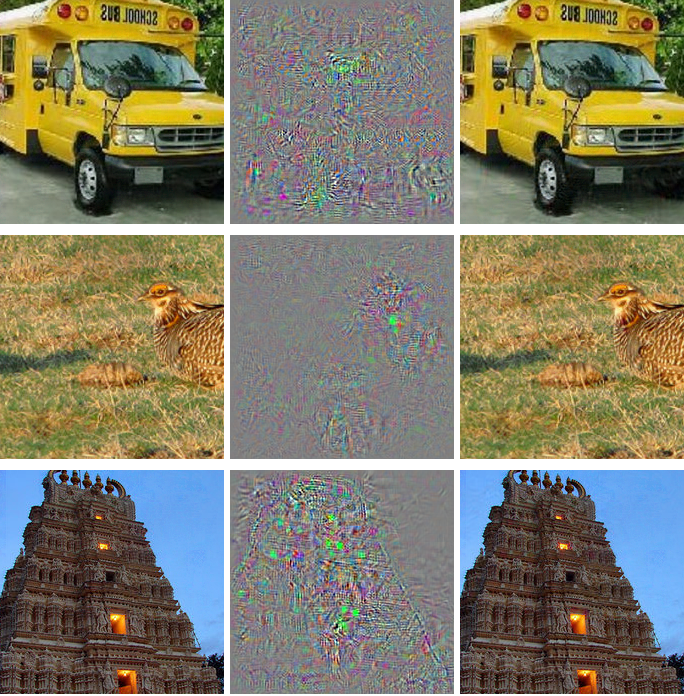
\includegraphics[width=7.3cm]{c1_figures/negative1.png}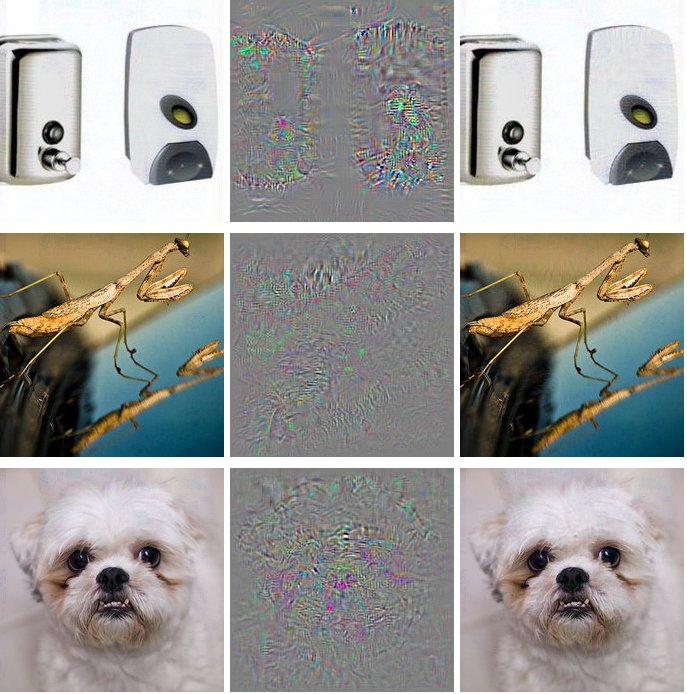
\includegraphics[width=7.3cm]{c1_figures/negative2.png}
    \caption{Natural Images are in columns 1 and 4, Adversarial images are in columns 3 and 6, and the difference between them (magnified by a factor of 10) is in columns 2 and 5. All images in columns 3 and 6 are classified by AlexNet as "Ostrich" \cite{Szegedy2013}}
    \label{fig:my_label}
\end{figure}

\section{Common Datasets}

The Dataset used above is known as ImageNet -- a large set of labeled images varying in size originally compiled for the ImageNet Large Scale Visual Recognition Challenge (ILSVRC). This dataset and its many subsets has become a standard for image classification and feature identification experiments. In the experiments that follow, ImageNet will be featured alongside the Modified National Institute of Standards and Technology (MNIST) dataset which is a database of hand written digits often used to develop image processing and character recognition systems. This dataset is much lower resolution than ImageNet and is therefore experiments run much more quickly on it and require less complex input/output.  

\section{Attack Techniques}
% TODO : Add massive carlini toolkit reference
\subsection{L-BFGS minimizing distortion}\label{lbfgs}

Szegedy et al. took advantage of the tools they had on hand for training neural networks to set up a box-constrained optimization problem whose approximated solution generates these targeted misclassifications. 


Let $f : \R^m \to \{1,...,k\}$ be a classifier and assume $f$ has an associated continuous loss function denoted by loss$_f : \R^m \times \{1,...,k\} \to \R^+$ and $l$ a target adversarial . \\
\textbf{ Minimize} $\Norm{r}_2$ subject to:
\begin{enumerate}[1.]
\item $f(x + r) = l$
\item $x + r \in [0,1]^m$
\end{enumerate}

The solution is approximated with L-BFGS (see Appendix \ref{appa}) as implemented in Pytorch or Keras. This technique yields examples that are close to their original counterparts in the $L^2$ sense.  \\

%Find the minimum $c > 0$ for which the minimizer $r$ of the following satisfies $f(x+r) = l$\\

%minimize $c|r| + $loss$_f(x+r,l)$ subject to $x + r \in [0,1]^m$.

\paragraph{L-BFGS: Mnist}
The following examples are prepared by implementing the above technique via pytorch on images from the Mnist dataset with FC200-200-10, a neural network with 2 hidden layers with 200 nodes each:
\begin{figure}[H]
\label{lbfgsa}
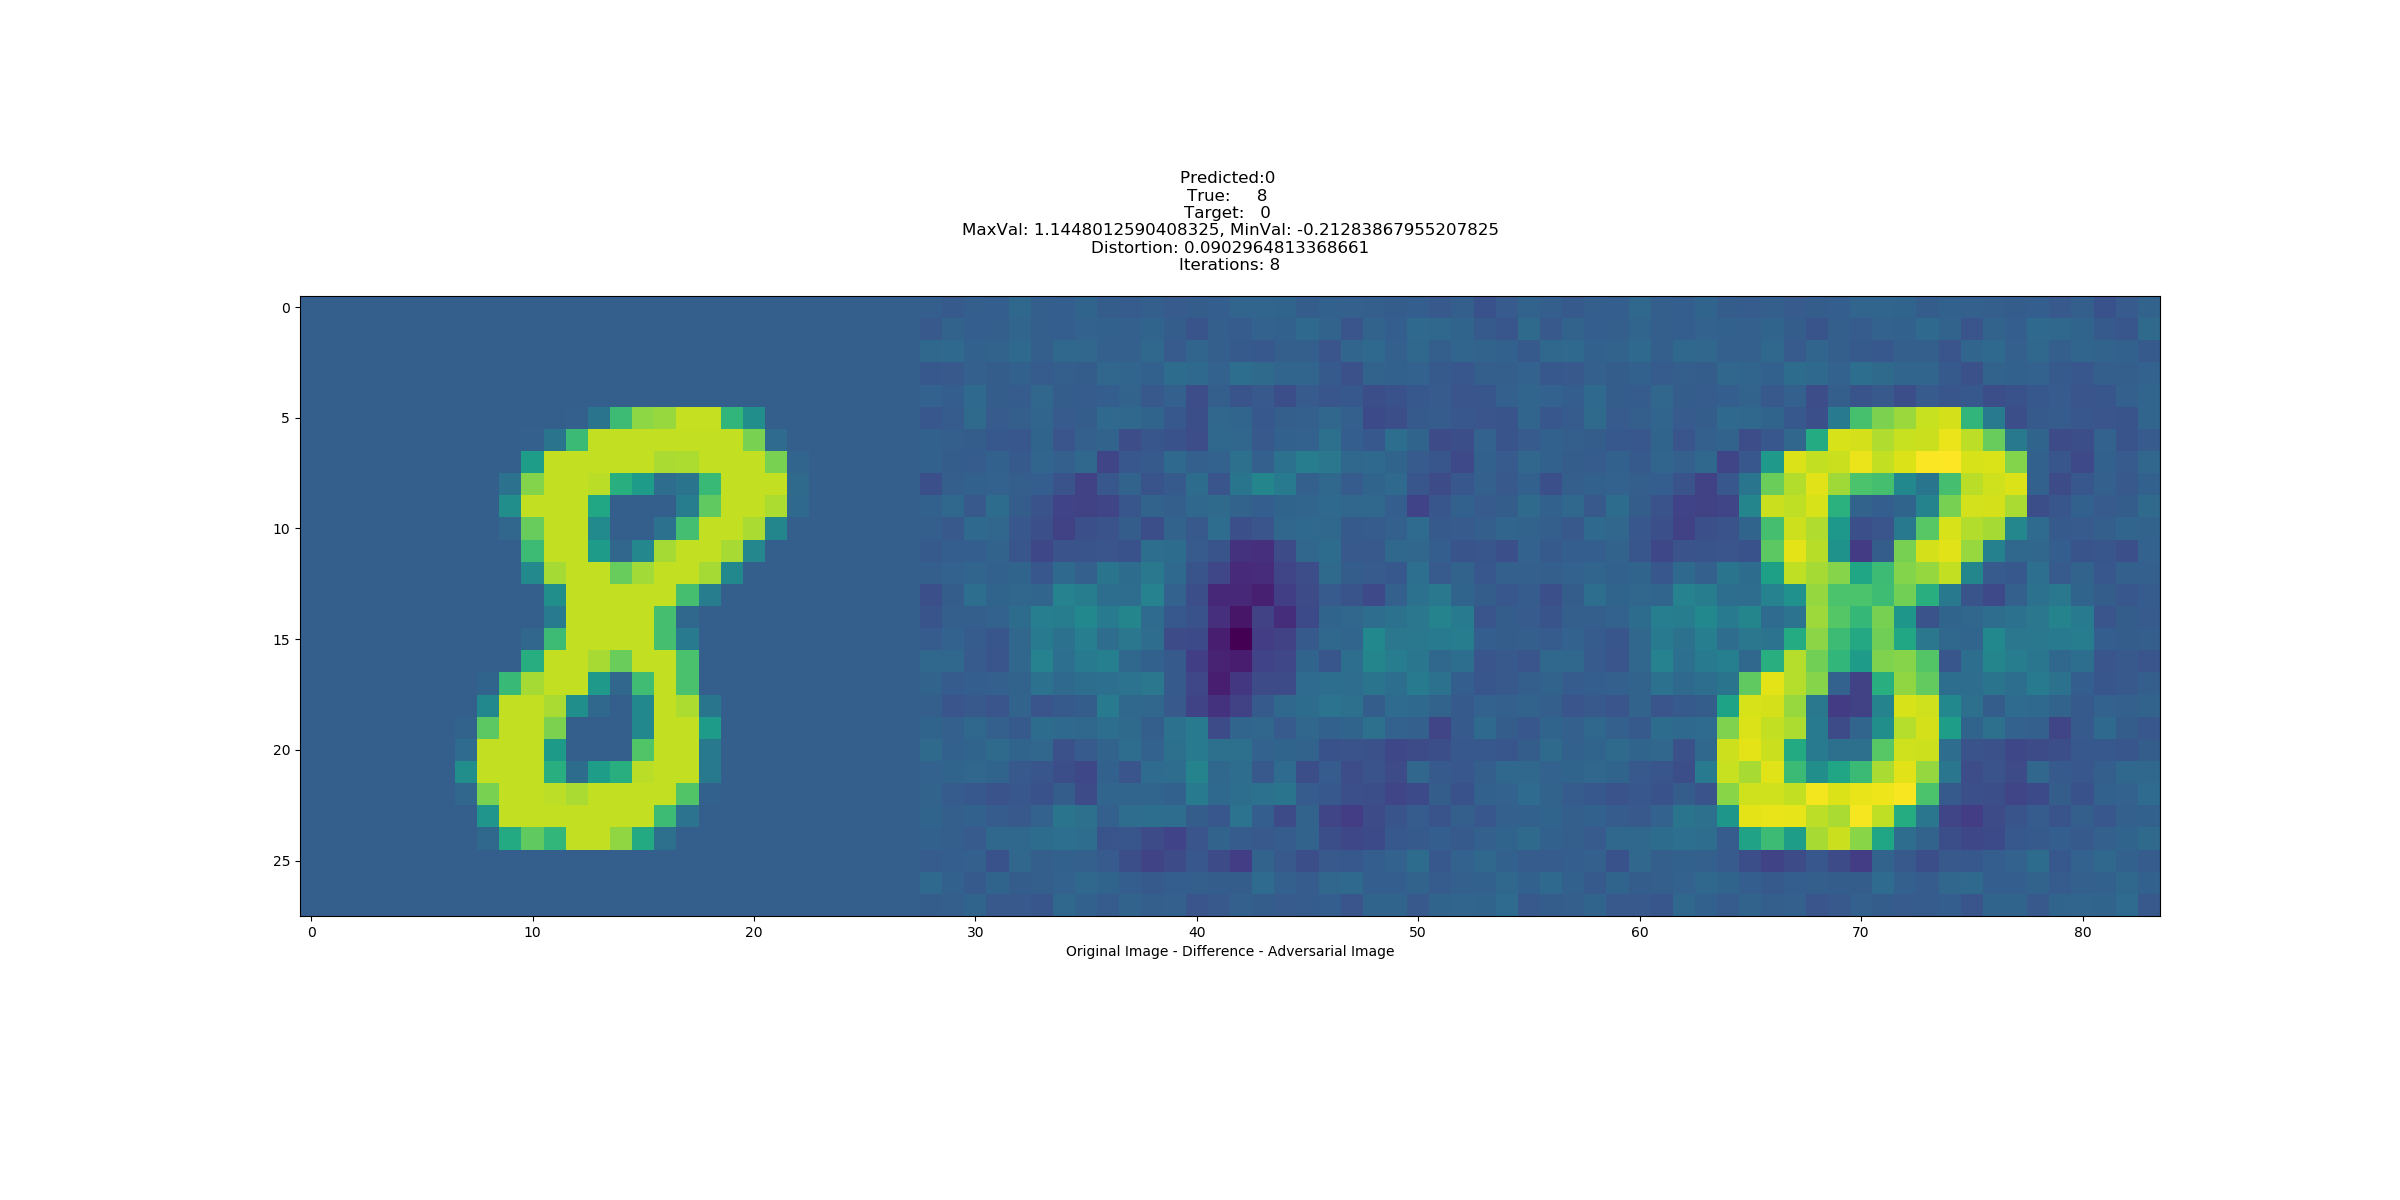
\includegraphics[trim=200 185 100 200, clip, width=7cm]{c1_figures/FC200-200-10-2448-O8-A0-attack_summary.png}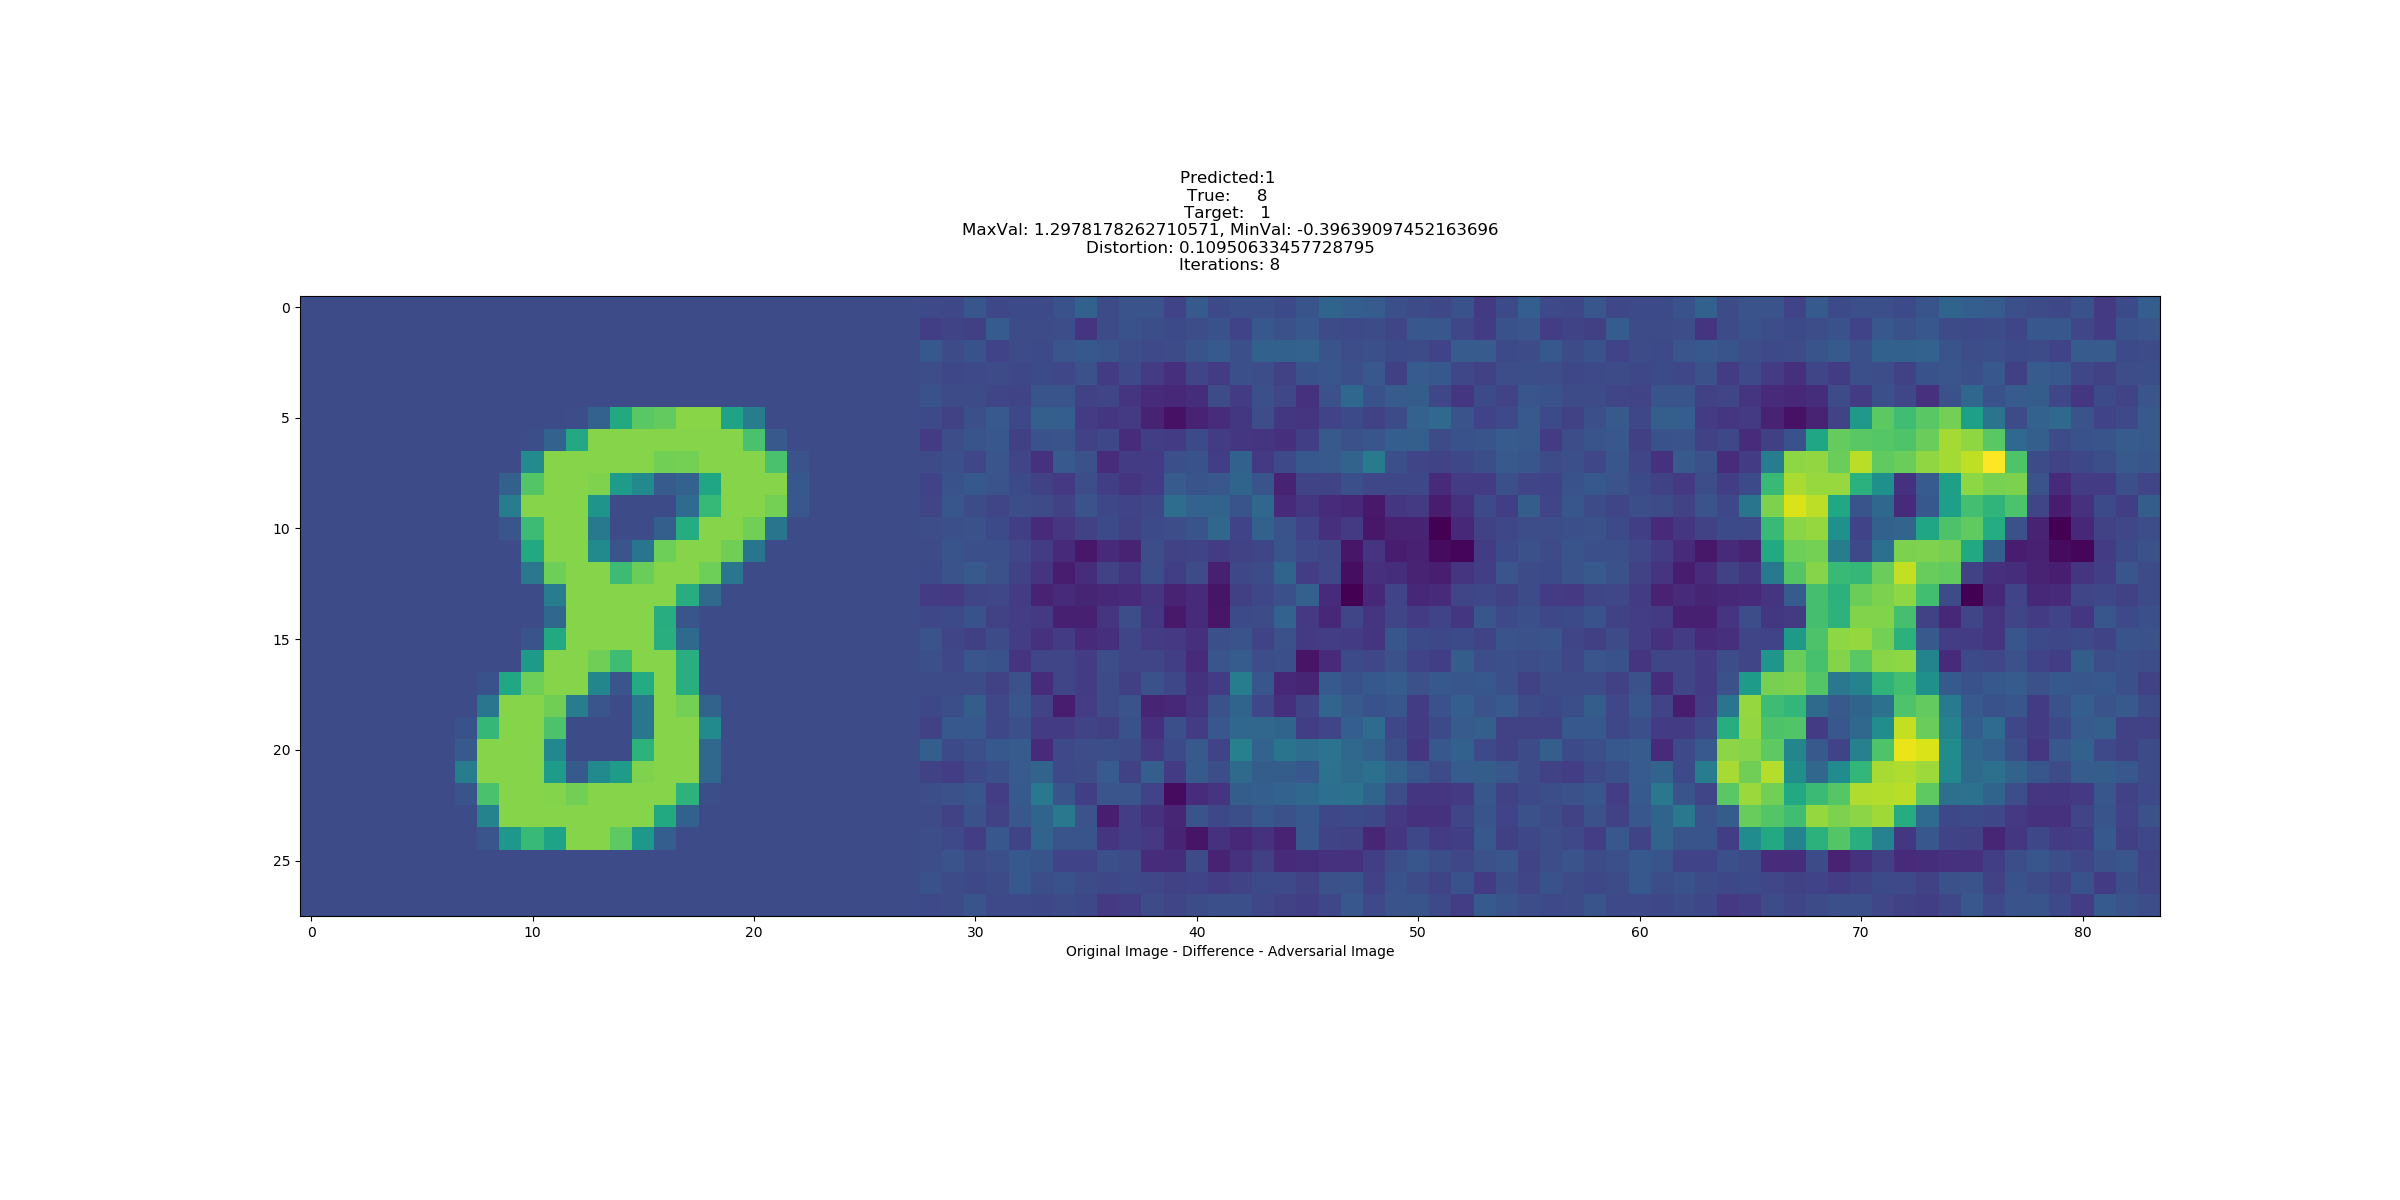
\includegraphics[trim=200 185 100 200, clip,width=7cm]{c1_figures/FC200-200-10-2448-O8-A1-attack_summary.png}
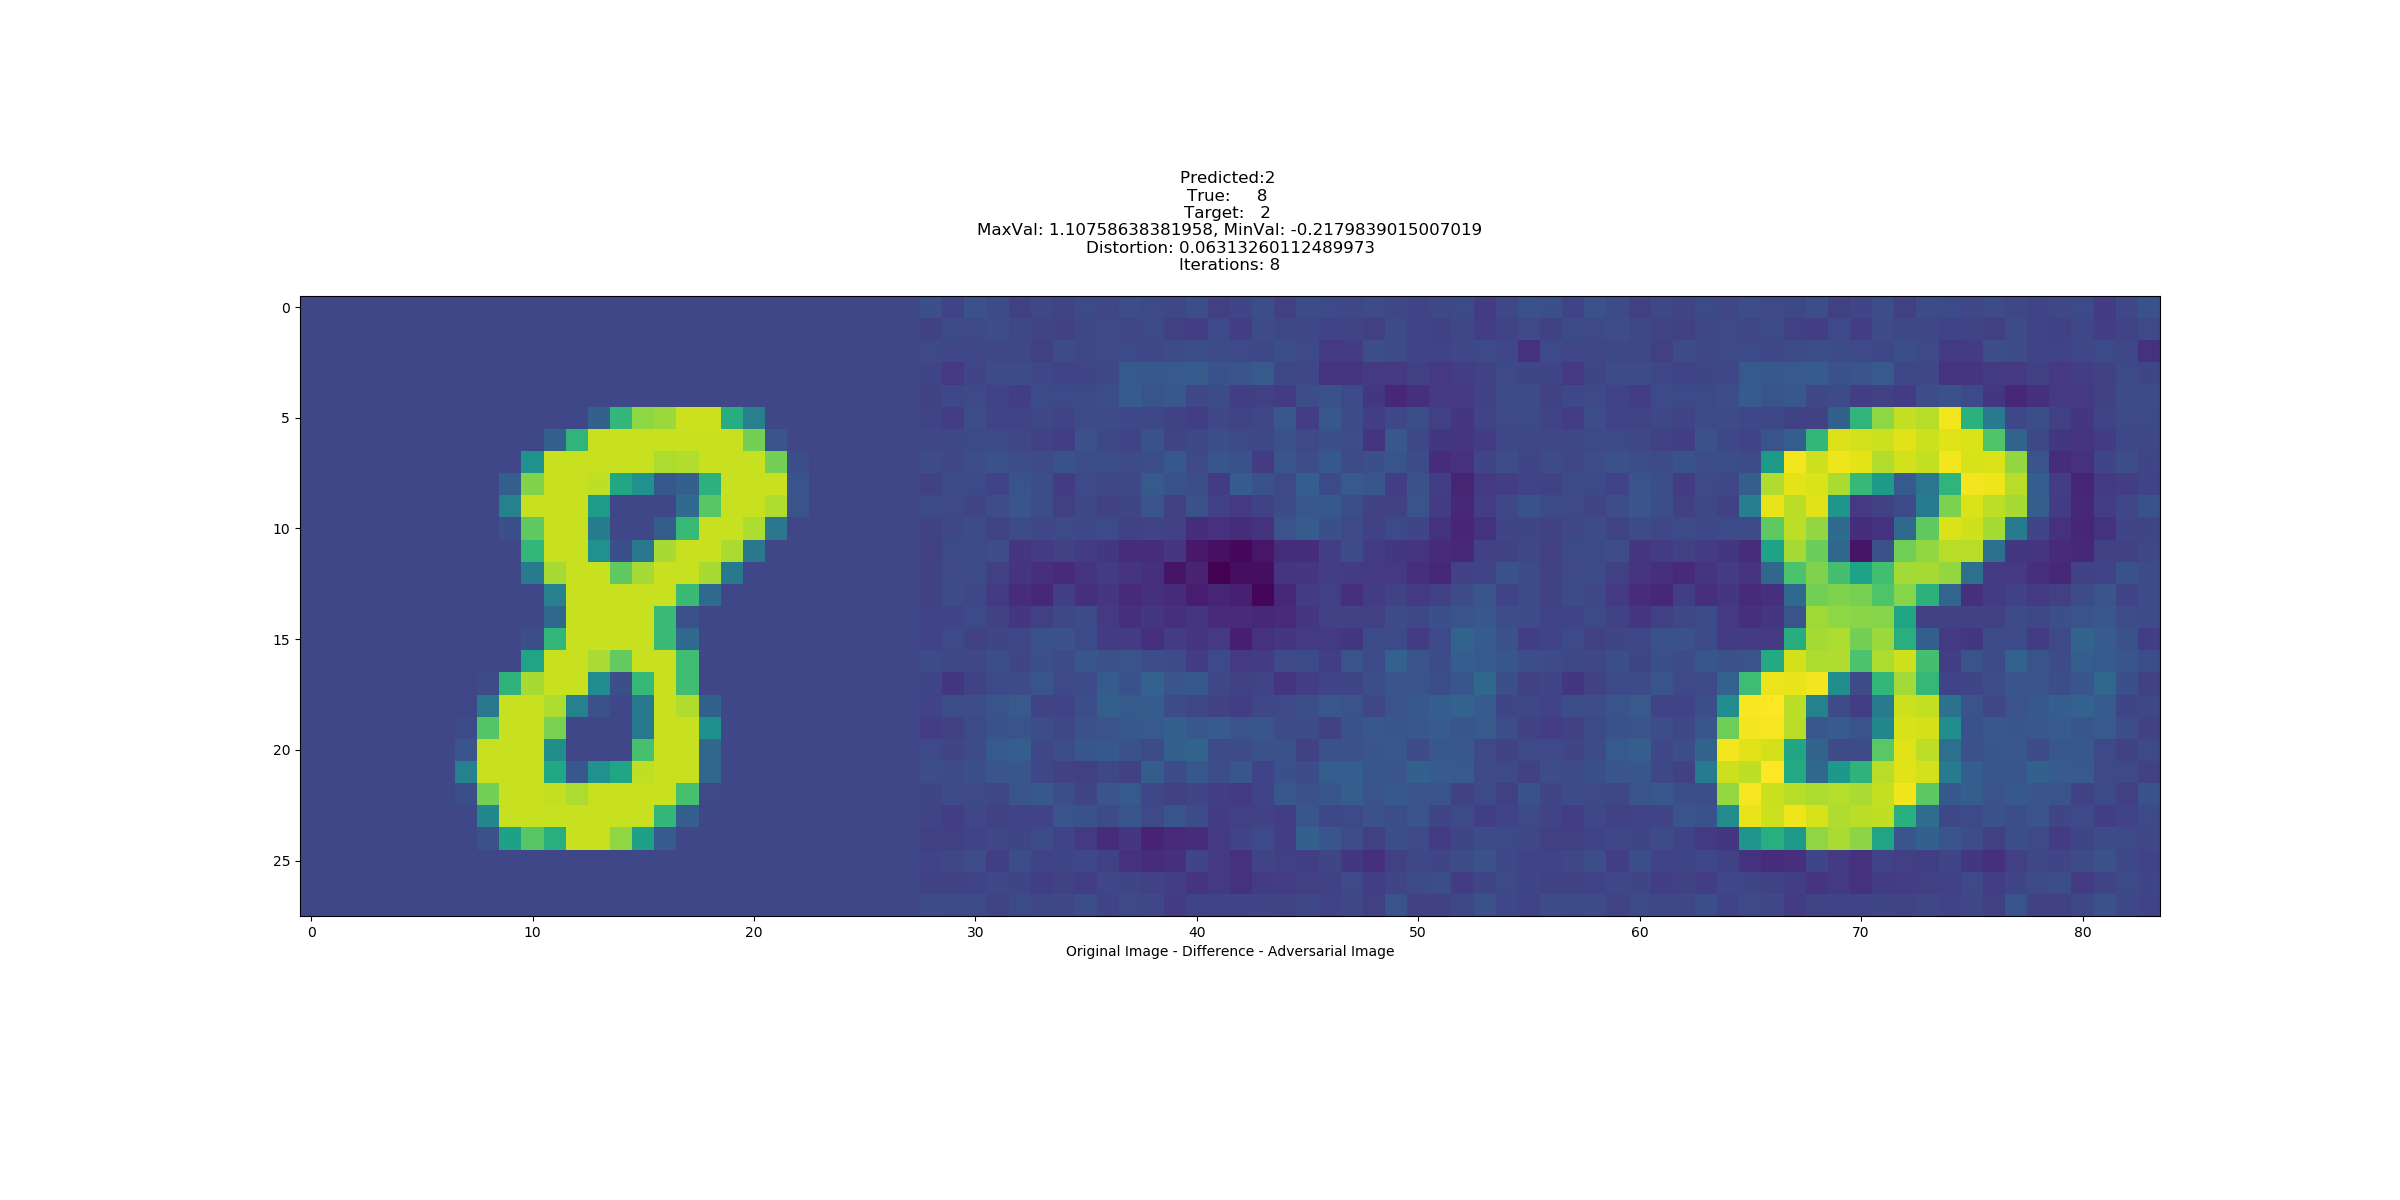
\includegraphics[trim=200 185 100 200, clip,width=7cm]{c1_figures/FC200-200-10-2448-O8-A2-attack_summary.png}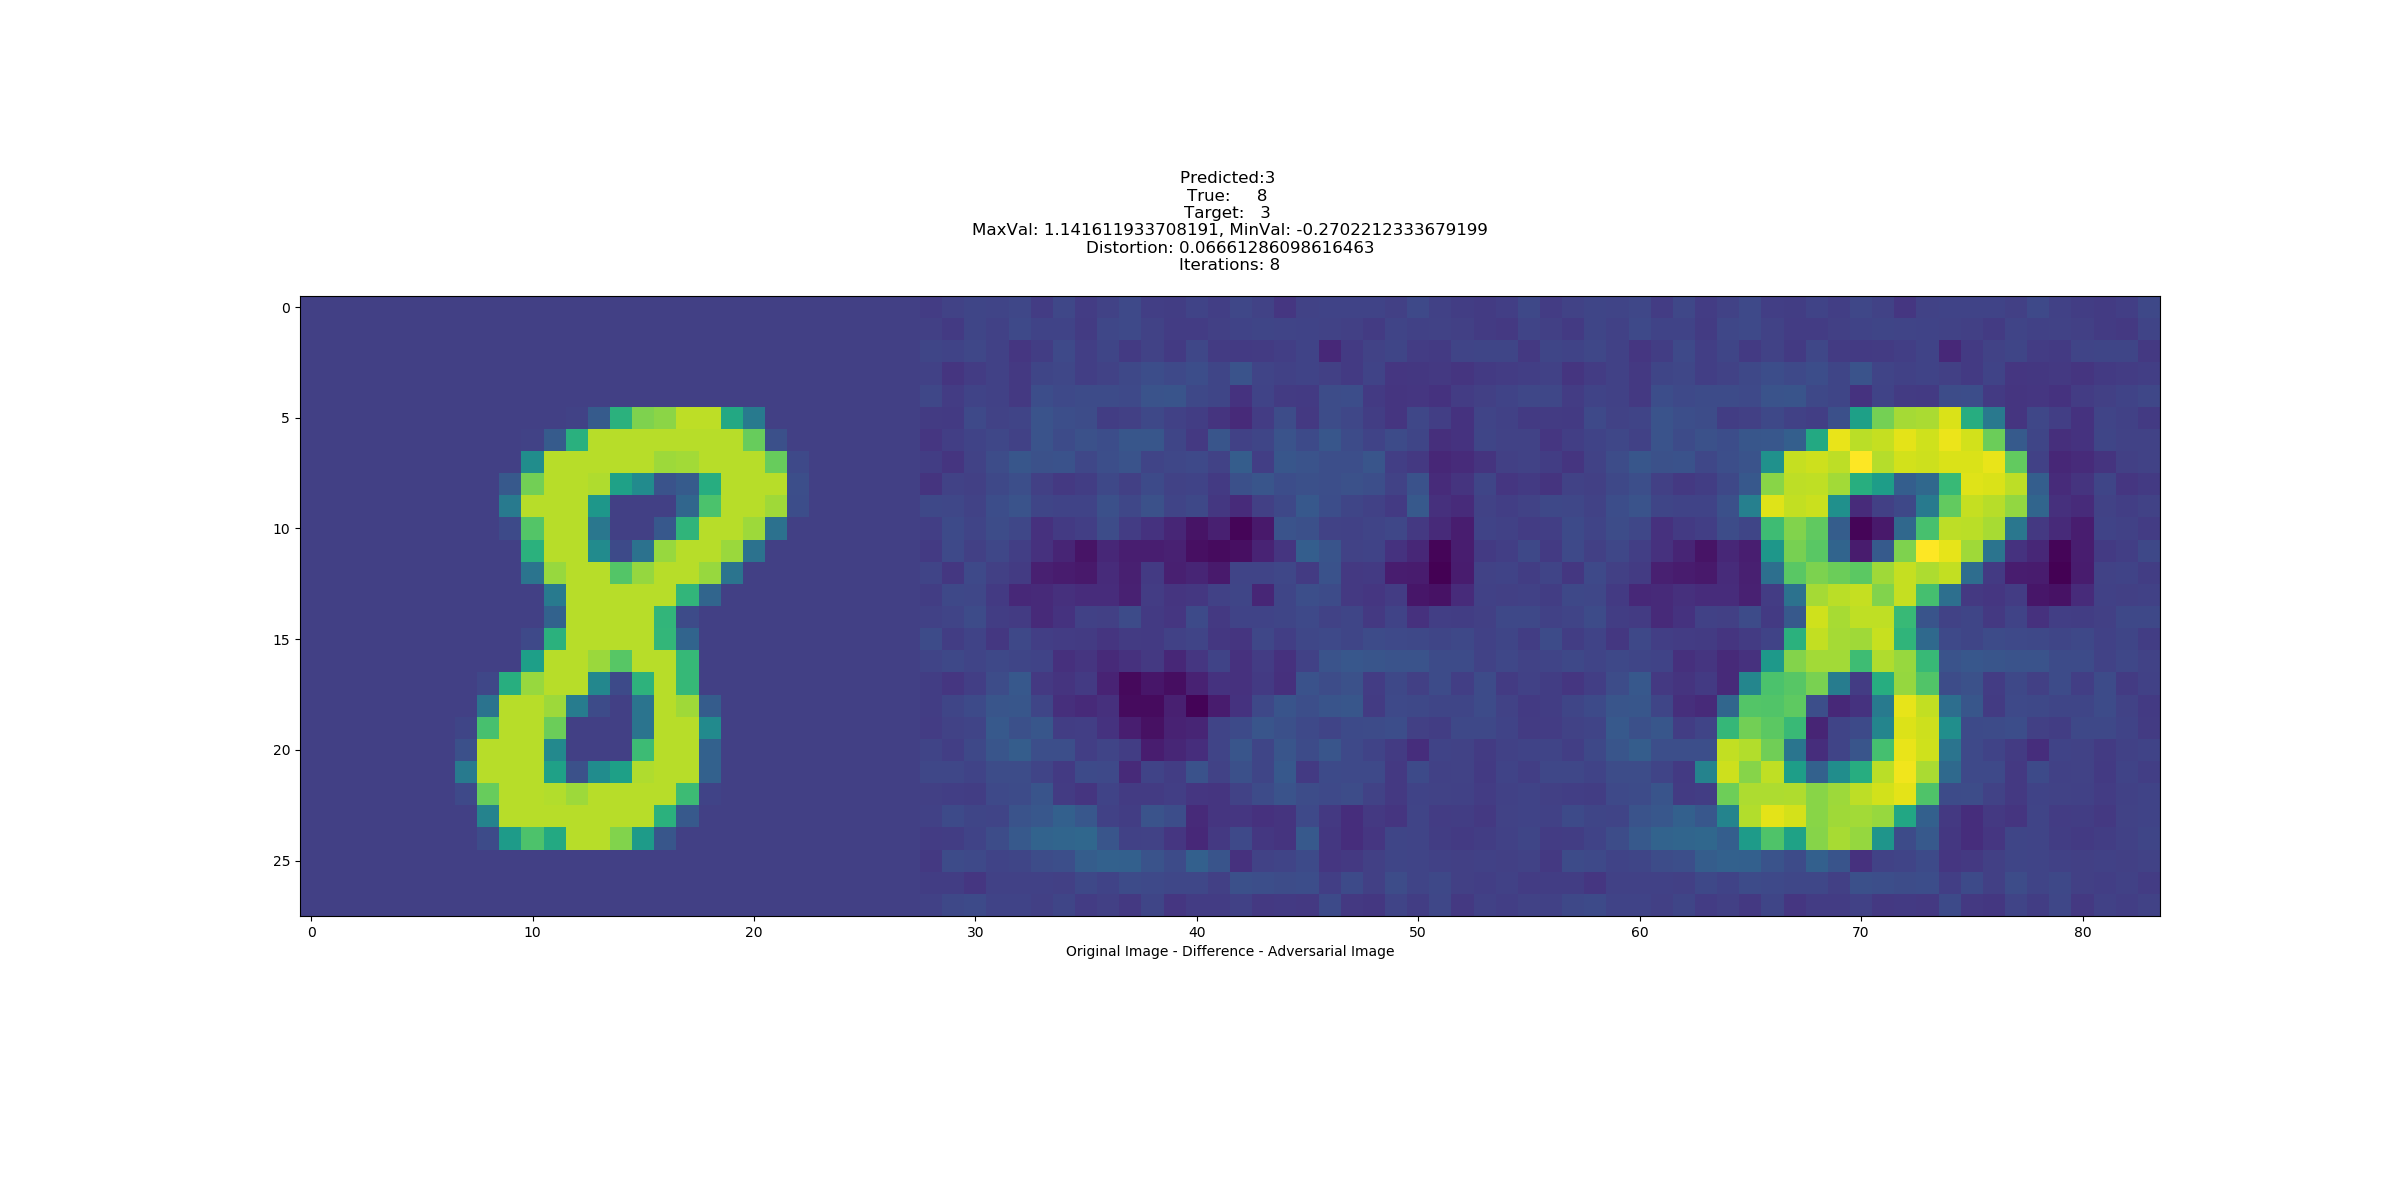
\includegraphics[trim=200 185 100 200, clip,width=7cm]{c1_figures/FC200-200-10-2448-O8-A3-attack_summary.png}
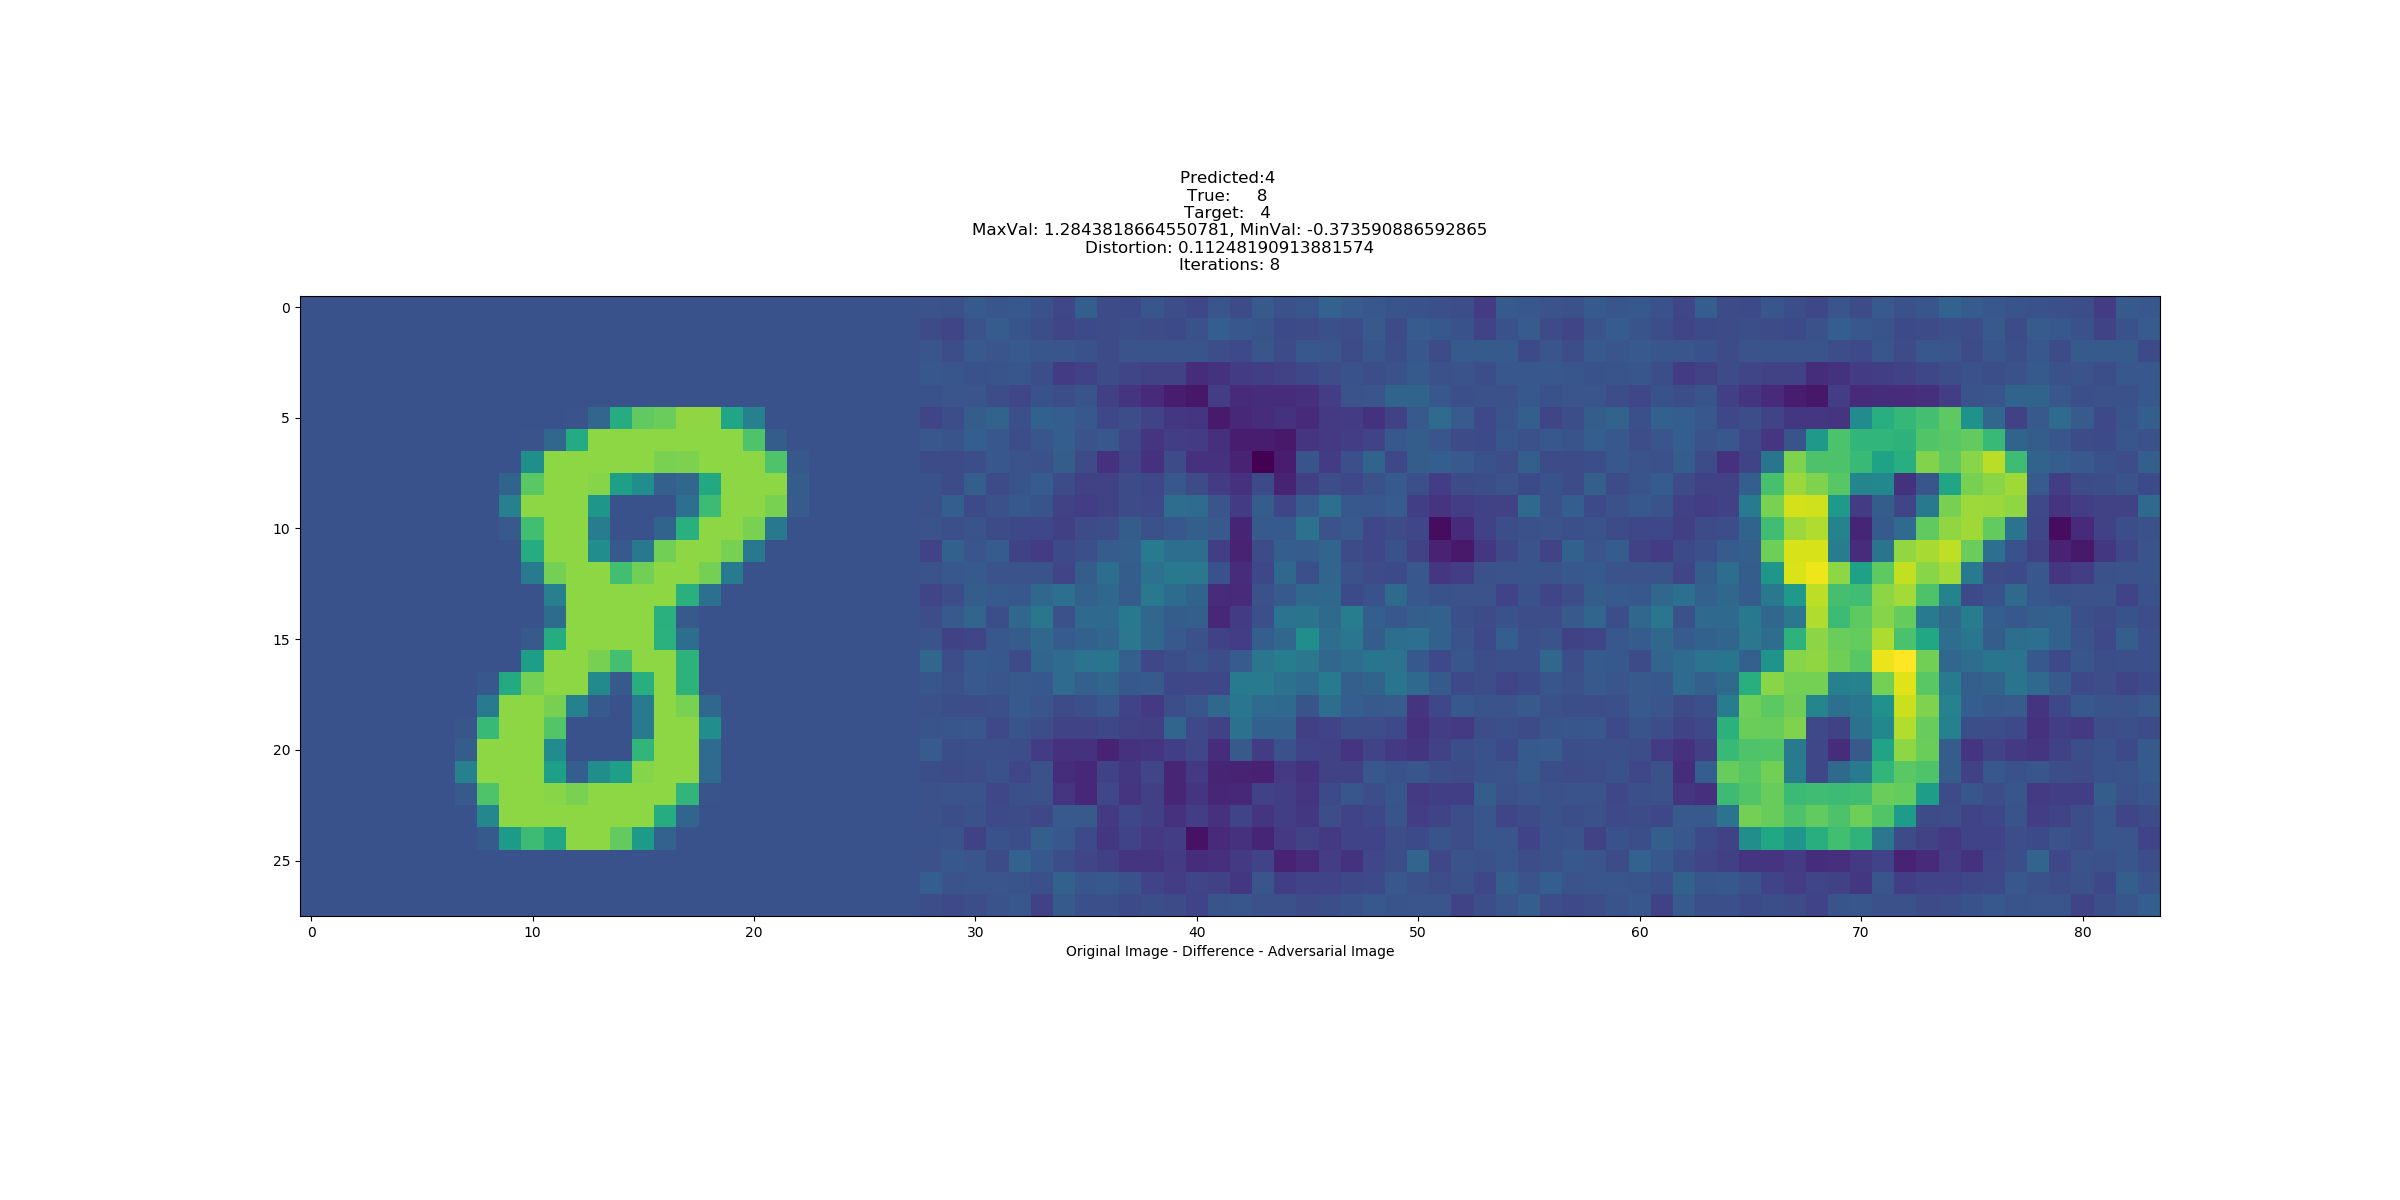
\includegraphics[trim=200 185 100 200, clip,width=7cm]{c1_figures/FC200-200-10-2448-O8-A4-attack_summary.png}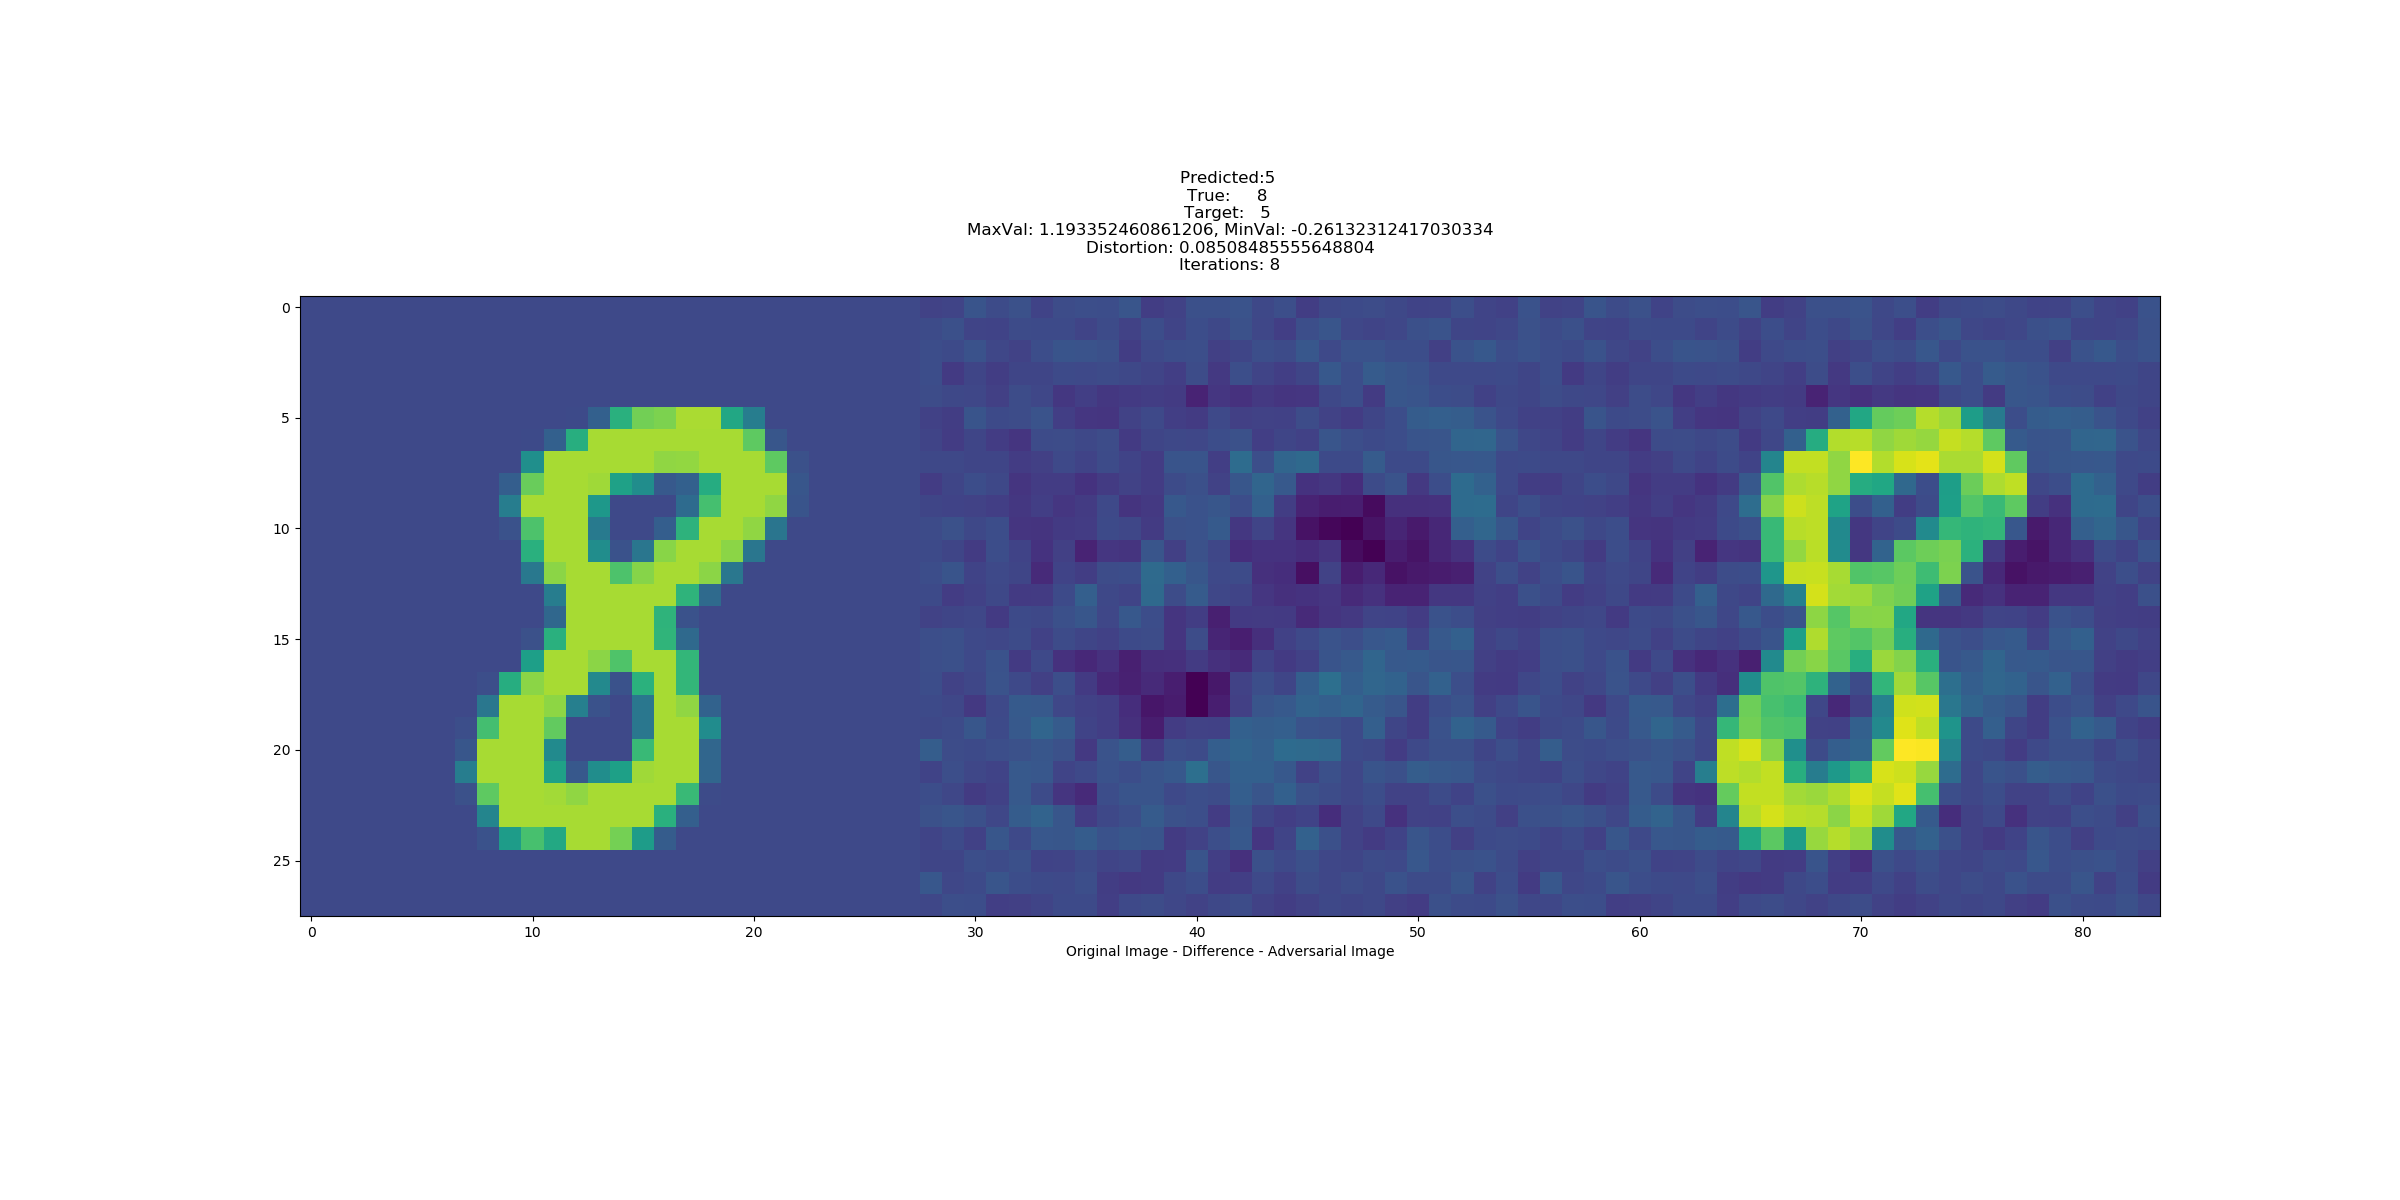
\includegraphics[trim=200 185 100 200, clip,width=7cm]{c1_figures/FC200-200-10-2448-O8-A5-attack_summary.png}
\caption{Original images on the left, Perturbation is in the middle, Adversarial Image (total of Original with Perturbation) is on the right. Column 1 shows an original 8 being perturbed to adversarial classes 0, 2, and 4. Column 2 shows adversarial classes 1, 3, and 5}
\end{figure}
Borrowing a metric from Szegedy et al to compare the magnitude of these distortions, we will define
\begin{definition}{Distortion is the $L^2$ norm of the difference between an original image and a perturbed image, divided by the square root of the number of pixels in the image: }
\[\sqrt{\dfrac{\sum_i \hat (x_i - x_i)^2}{n}}\]
\end{definition}
Distortion is $L^2$ magnitude normalized by the square-root of the number of dimensions so that values can be compared for modeling problems with differing numbers of dimensions. 

The 900 examples generated for the network above had an average distortion of 0.089 with the following distribution of distortions, given in figure 3.

\begin{figure}[H]
\label{lbfgsh}
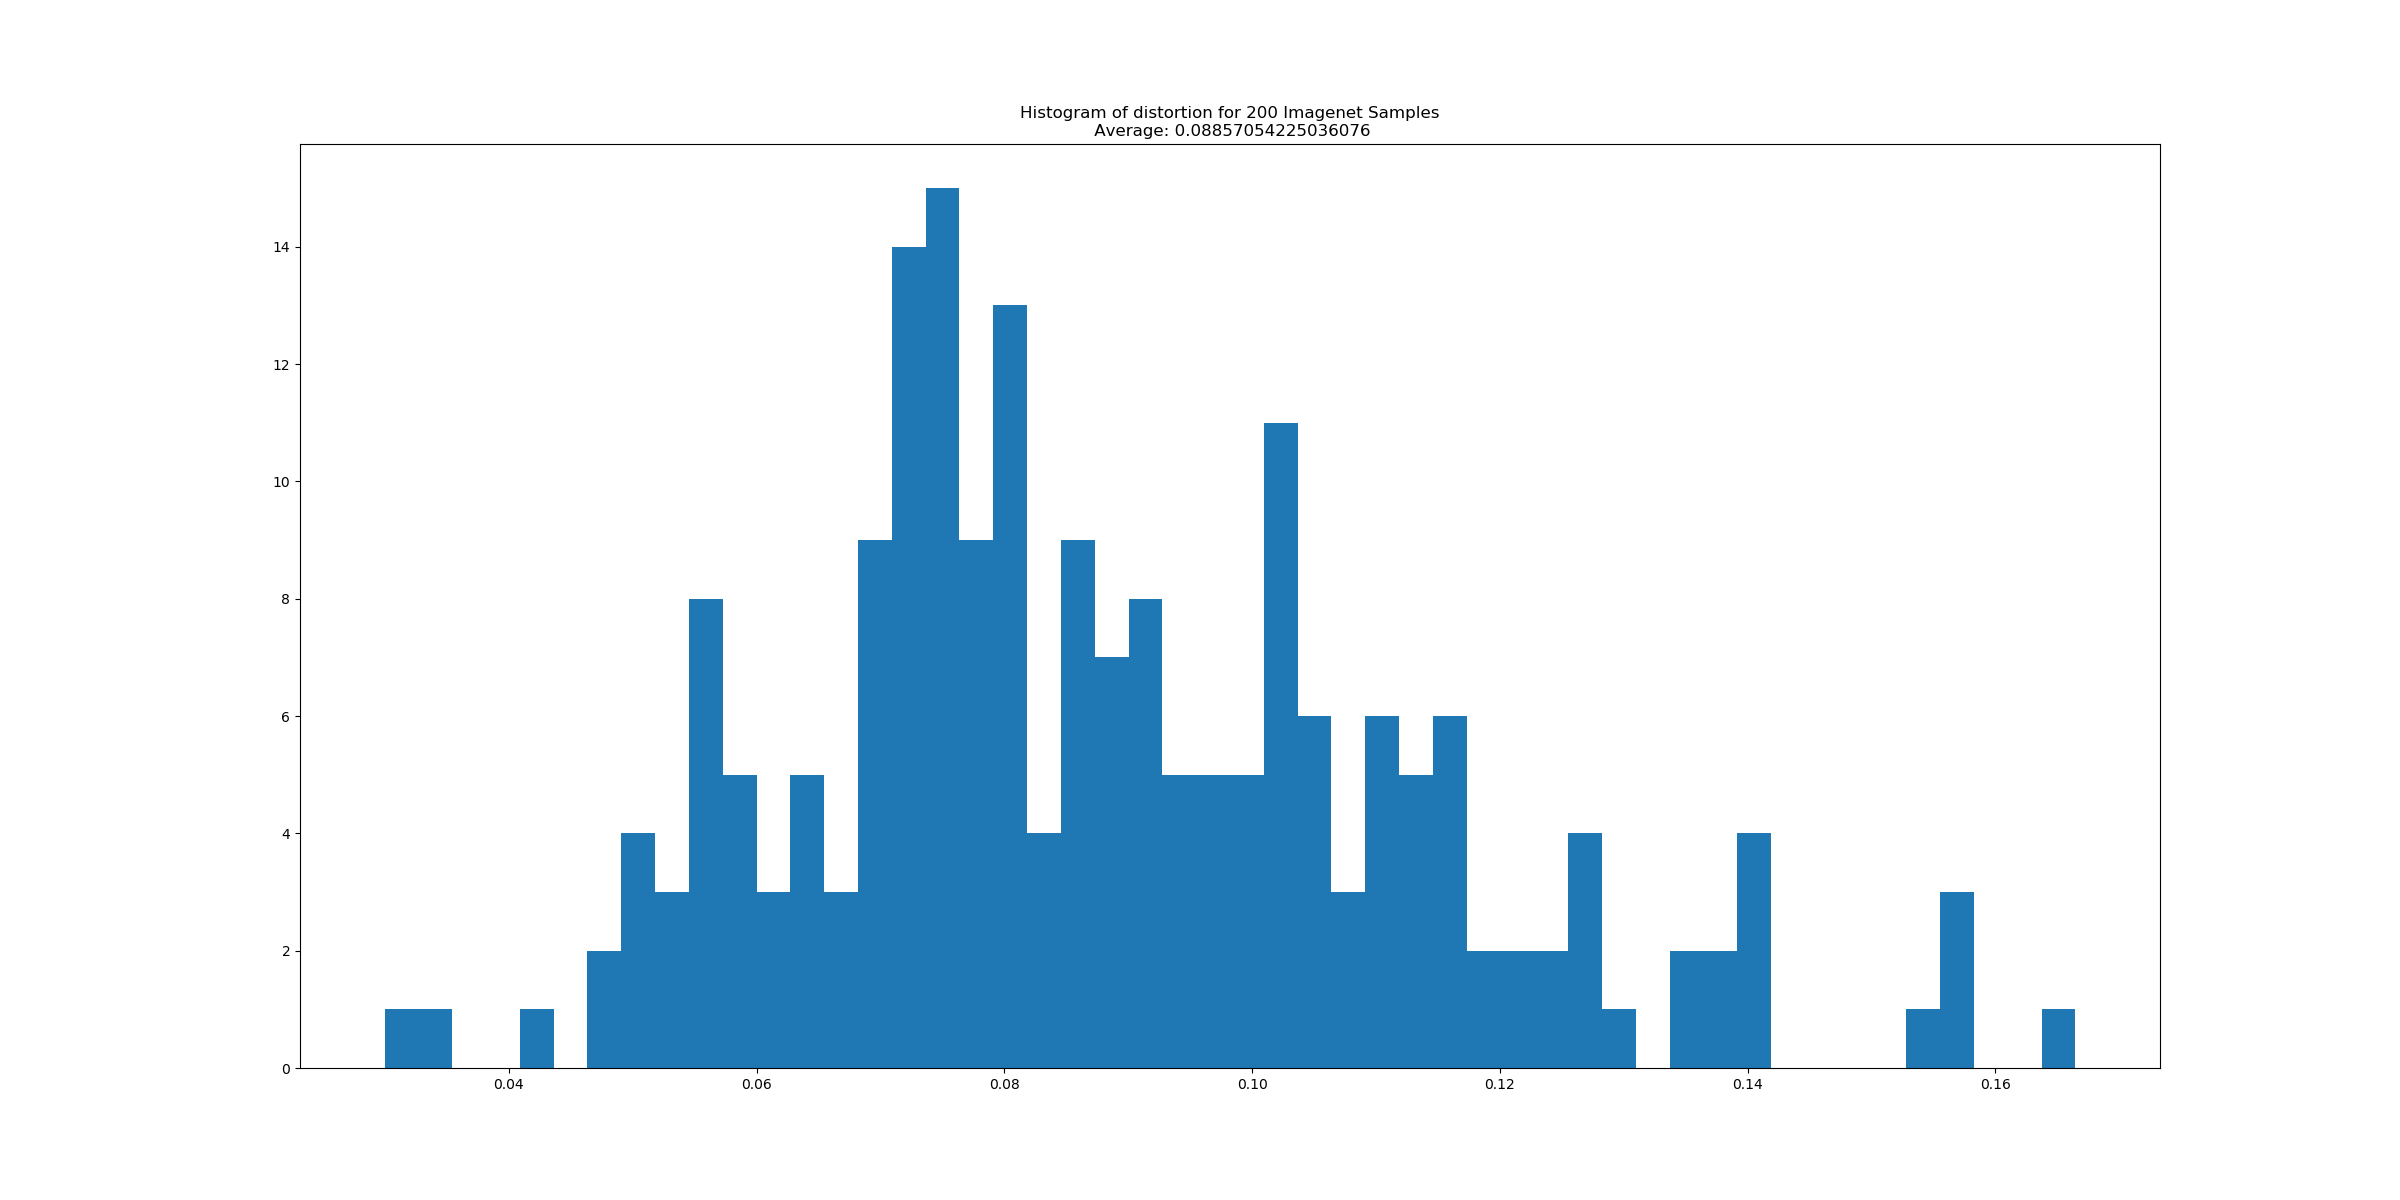
\includegraphics[trim=200 80 100 100, clip, width=16cm]{c1_figures/FC200-200-10-distortion_hist.png}
\caption{A histogram of the distortion measured for each of 900 adversarial examples generated using L-BFGS against the FC-200-200-10 network on Mnist. Mean distortion is 0.089.}
\end{figure}

\paragraph{L-BFGS: ImageNet}
\label{lbfgs-s}
We also tried to replicate \cite{Szegedy2013}'s results on ImageNet. Attacking VGG16, a well known model from the ILSVRC-2014 competition \cite{simonyan2014very}, on ImageNet images with the same technique generates the examples in figure 4: 

\begin{figure}[H]
\label{lbfgsis}
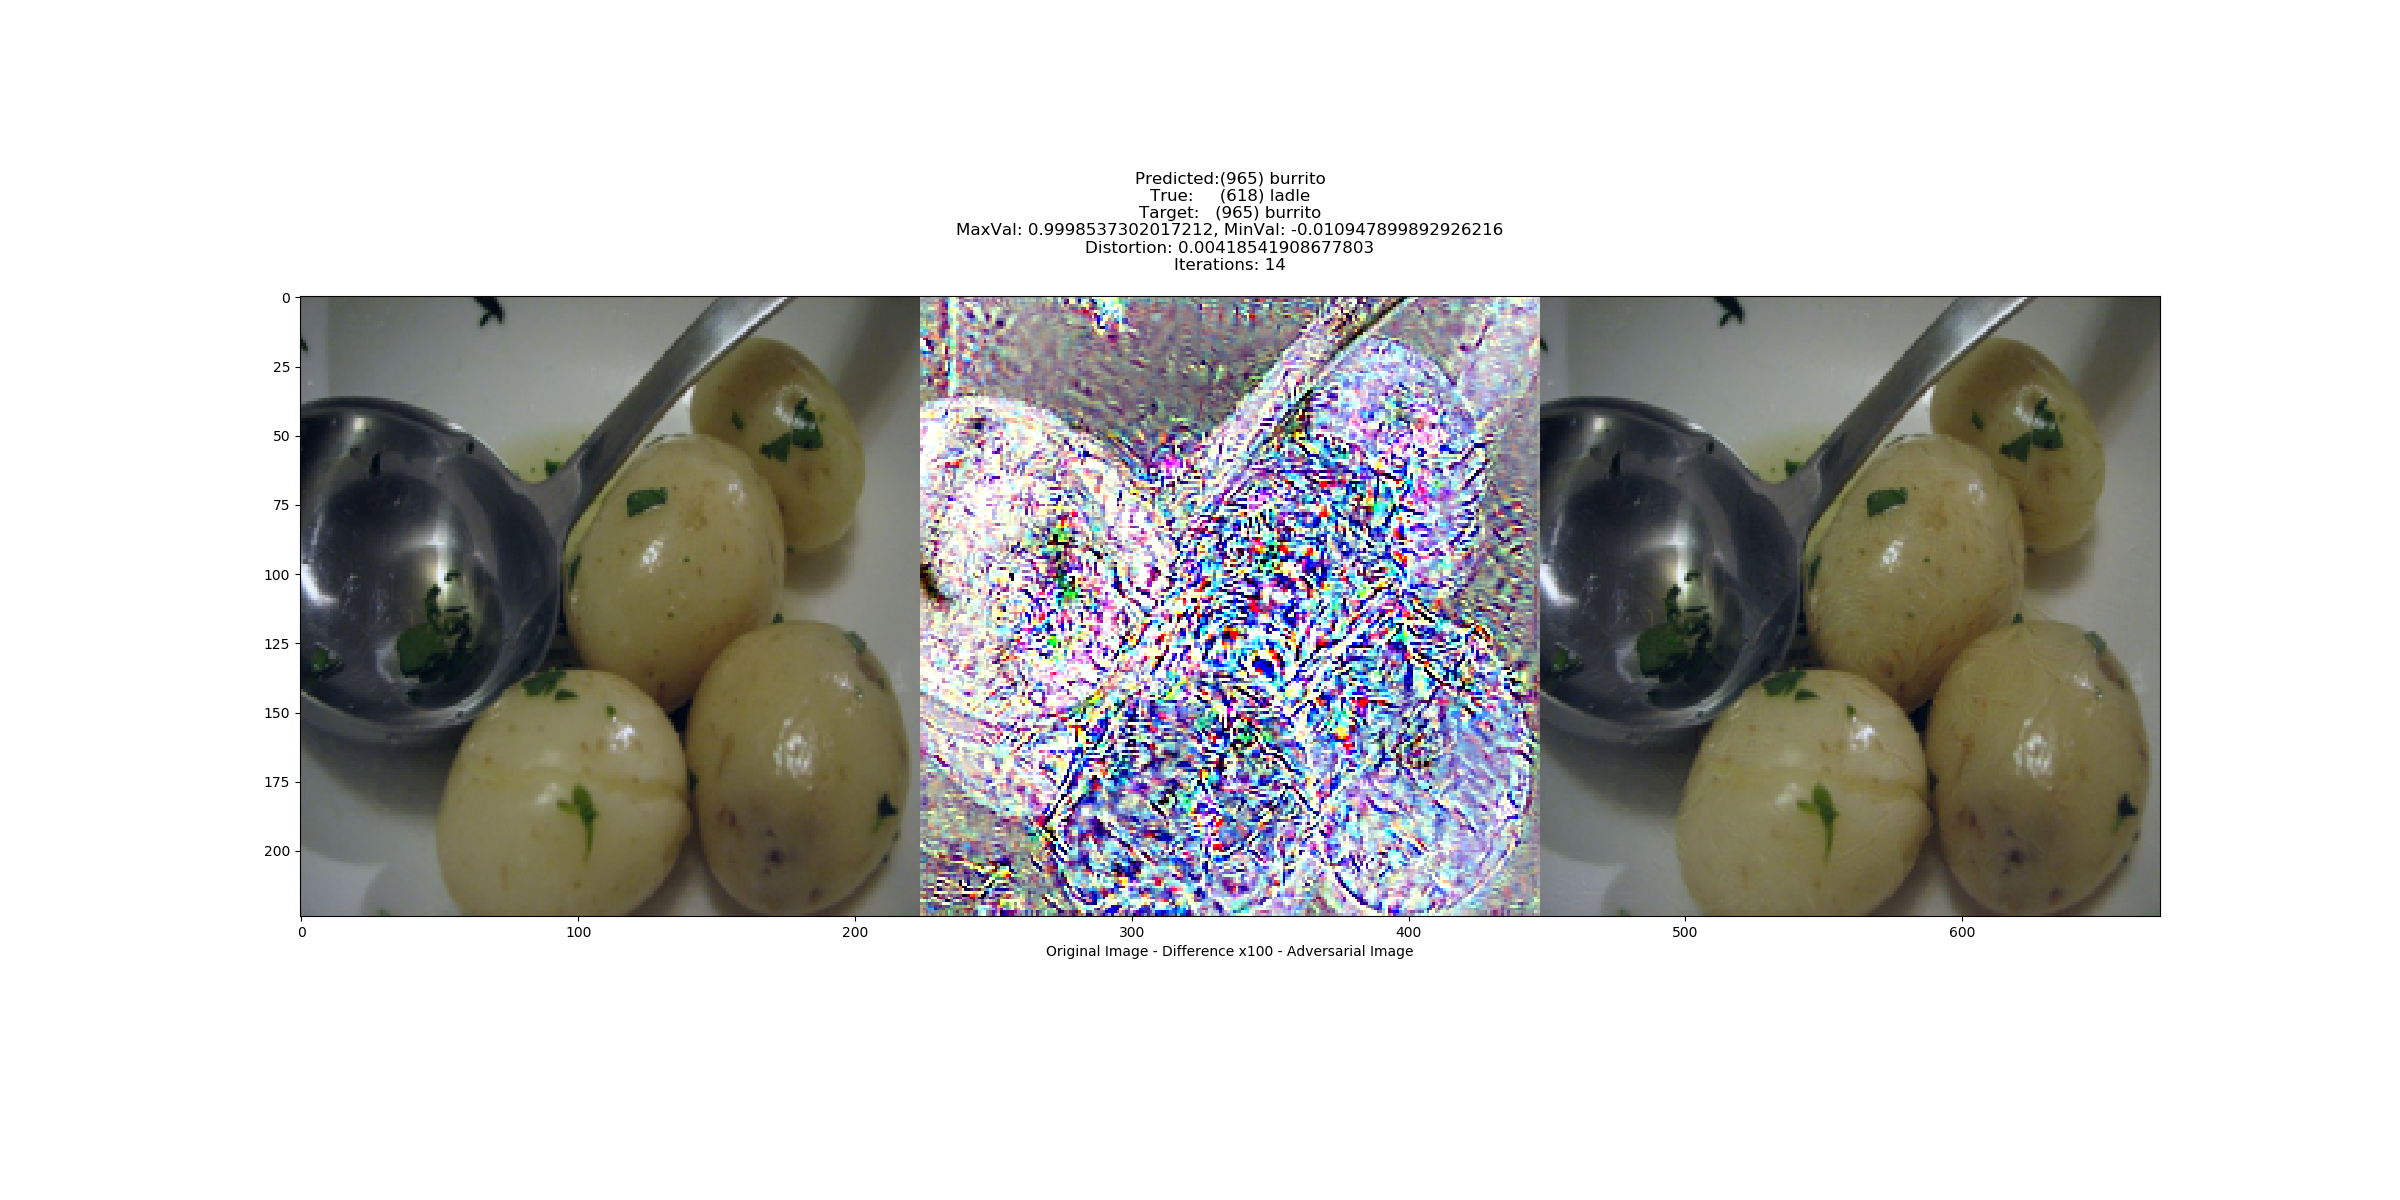
\includegraphics[trim=200 185 100 200, clip, width=8cm]{c1_figures/vgg16-ILSVRC2012_val_00039098-O722-A965-attack_summary.png}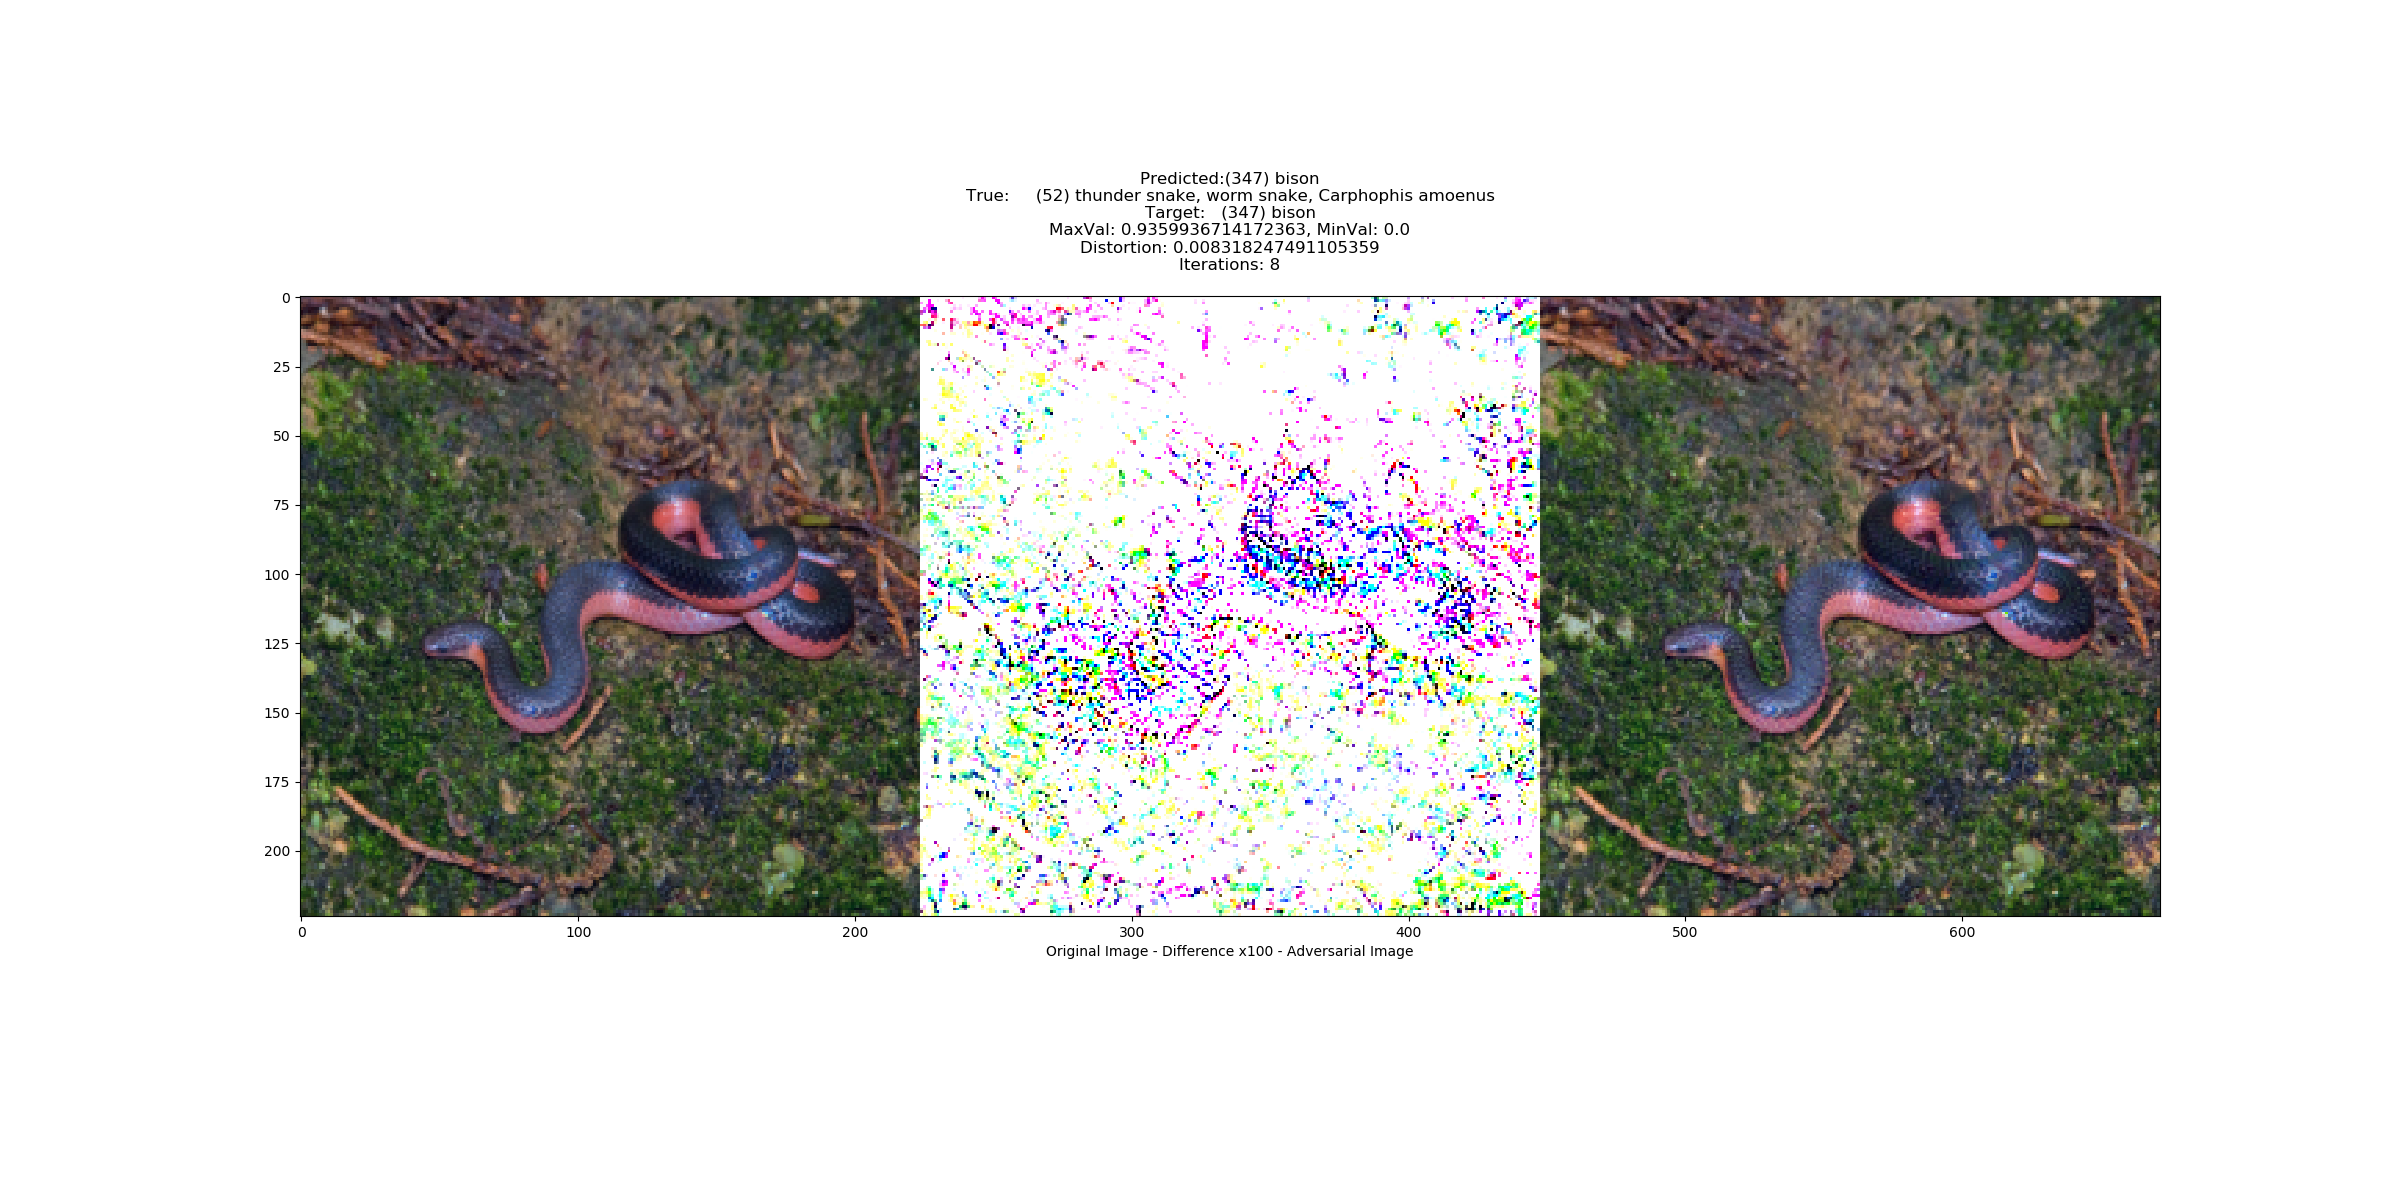
\includegraphics[trim=200 185 100 200, clip, width=8cm]{c1_figures/vgg16-ILSVRC2012_val_00027142-O52-A347-attack_summary.png}
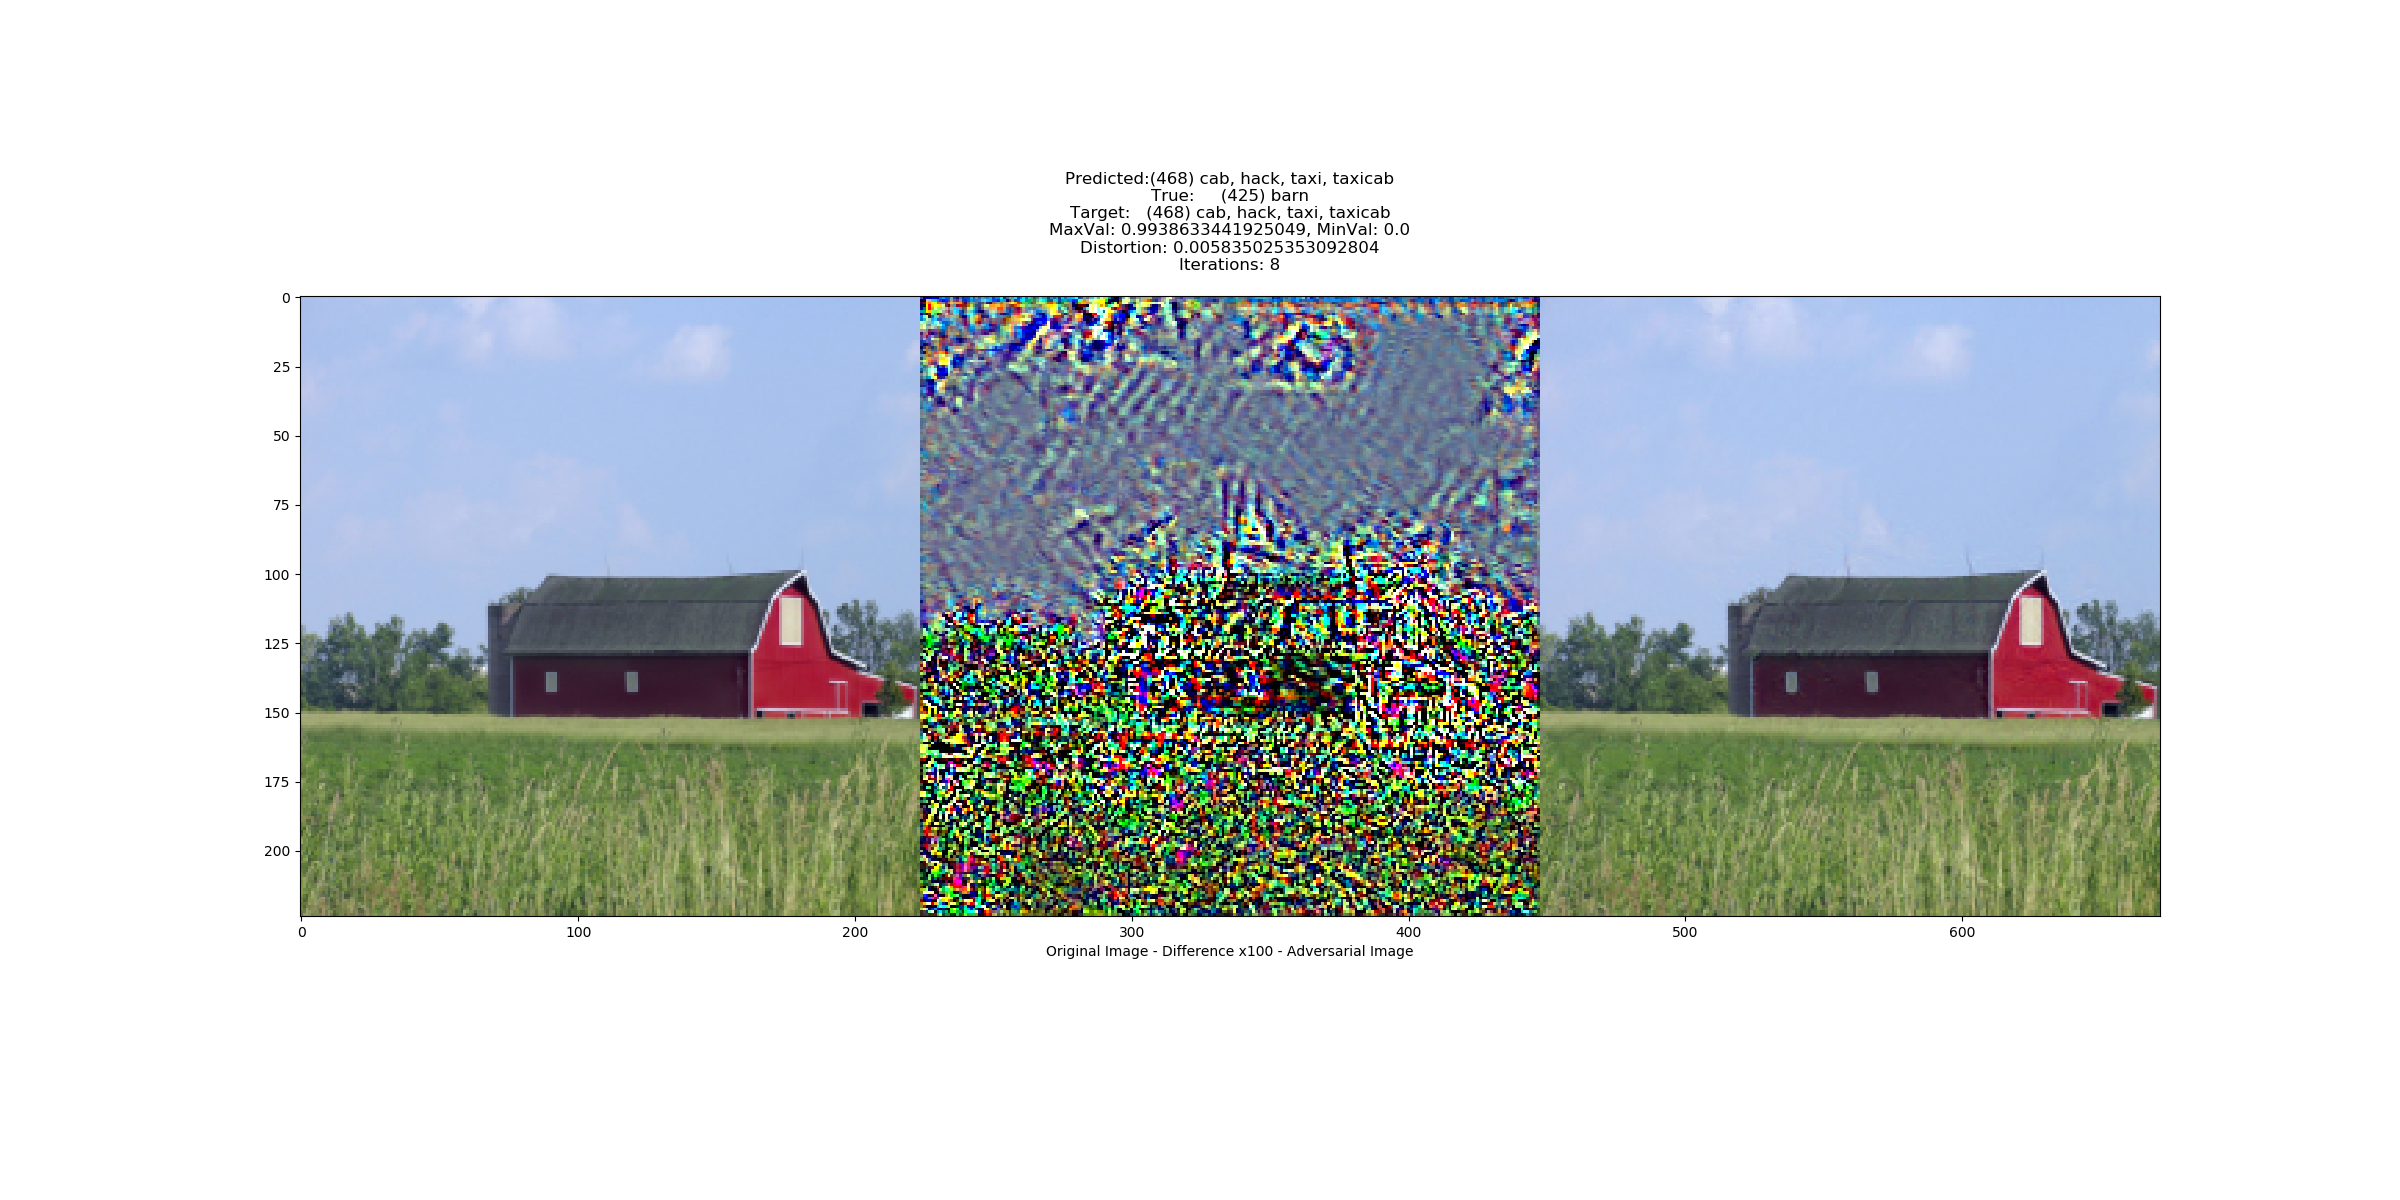
\includegraphics[trim=200 185 100 200, clip, width=8cm]{c1_figures/vgg16-ILSVRC2012_val_00029901-O425-A468-attack_summary.png}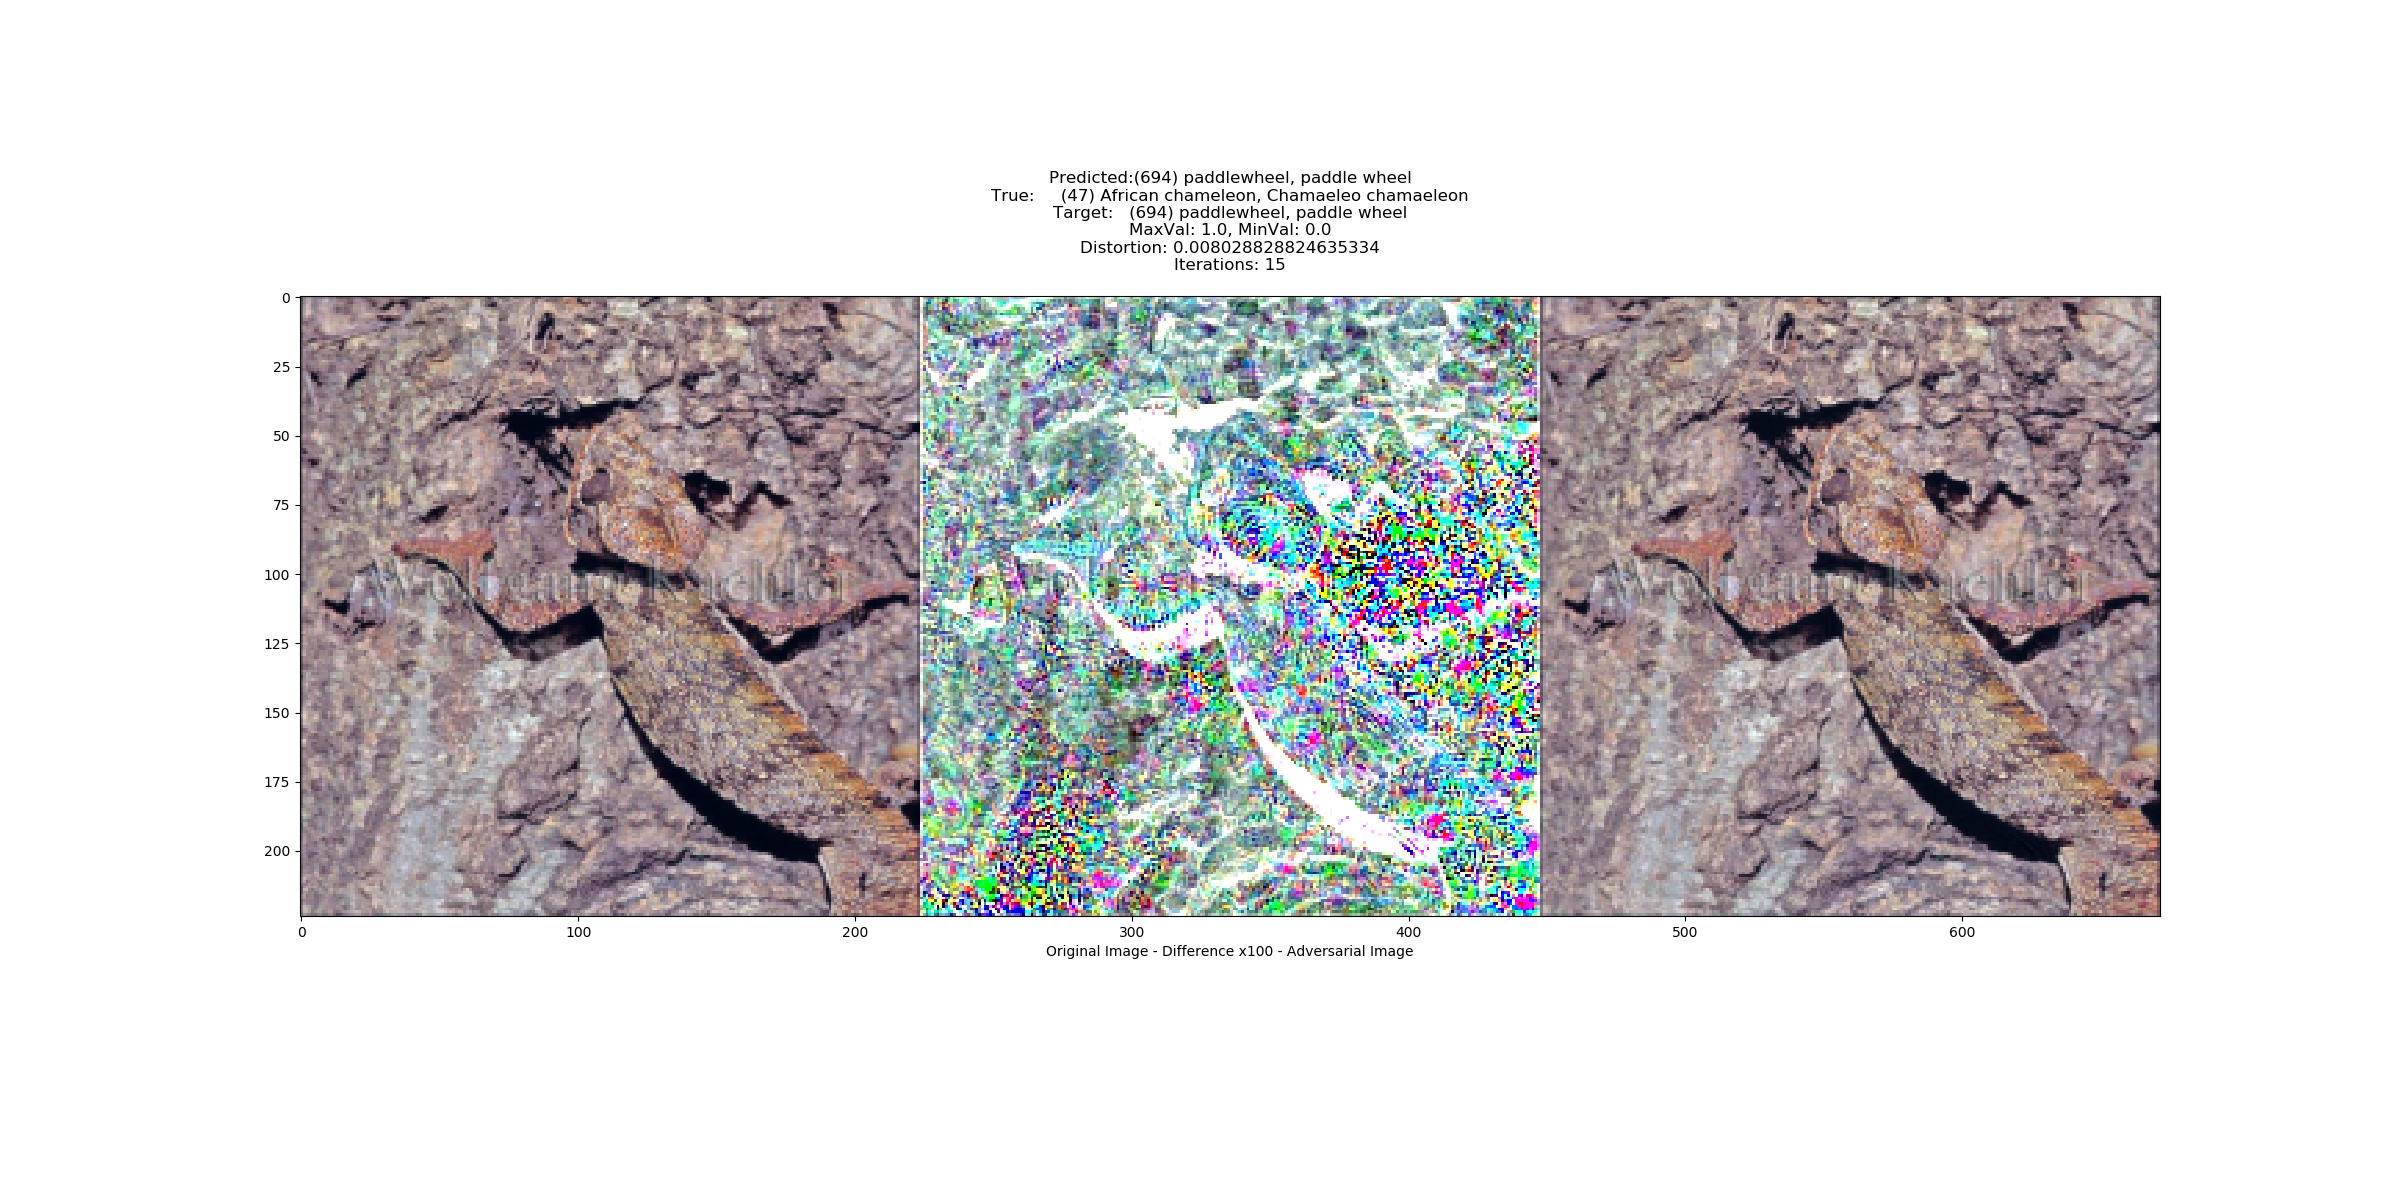
\includegraphics[trim=200 185 100 200, clip, width=8cm]{c1_figures/ILSVRC2012_val_00001375-Otensor([42])-A694-attack_summary.png}
% 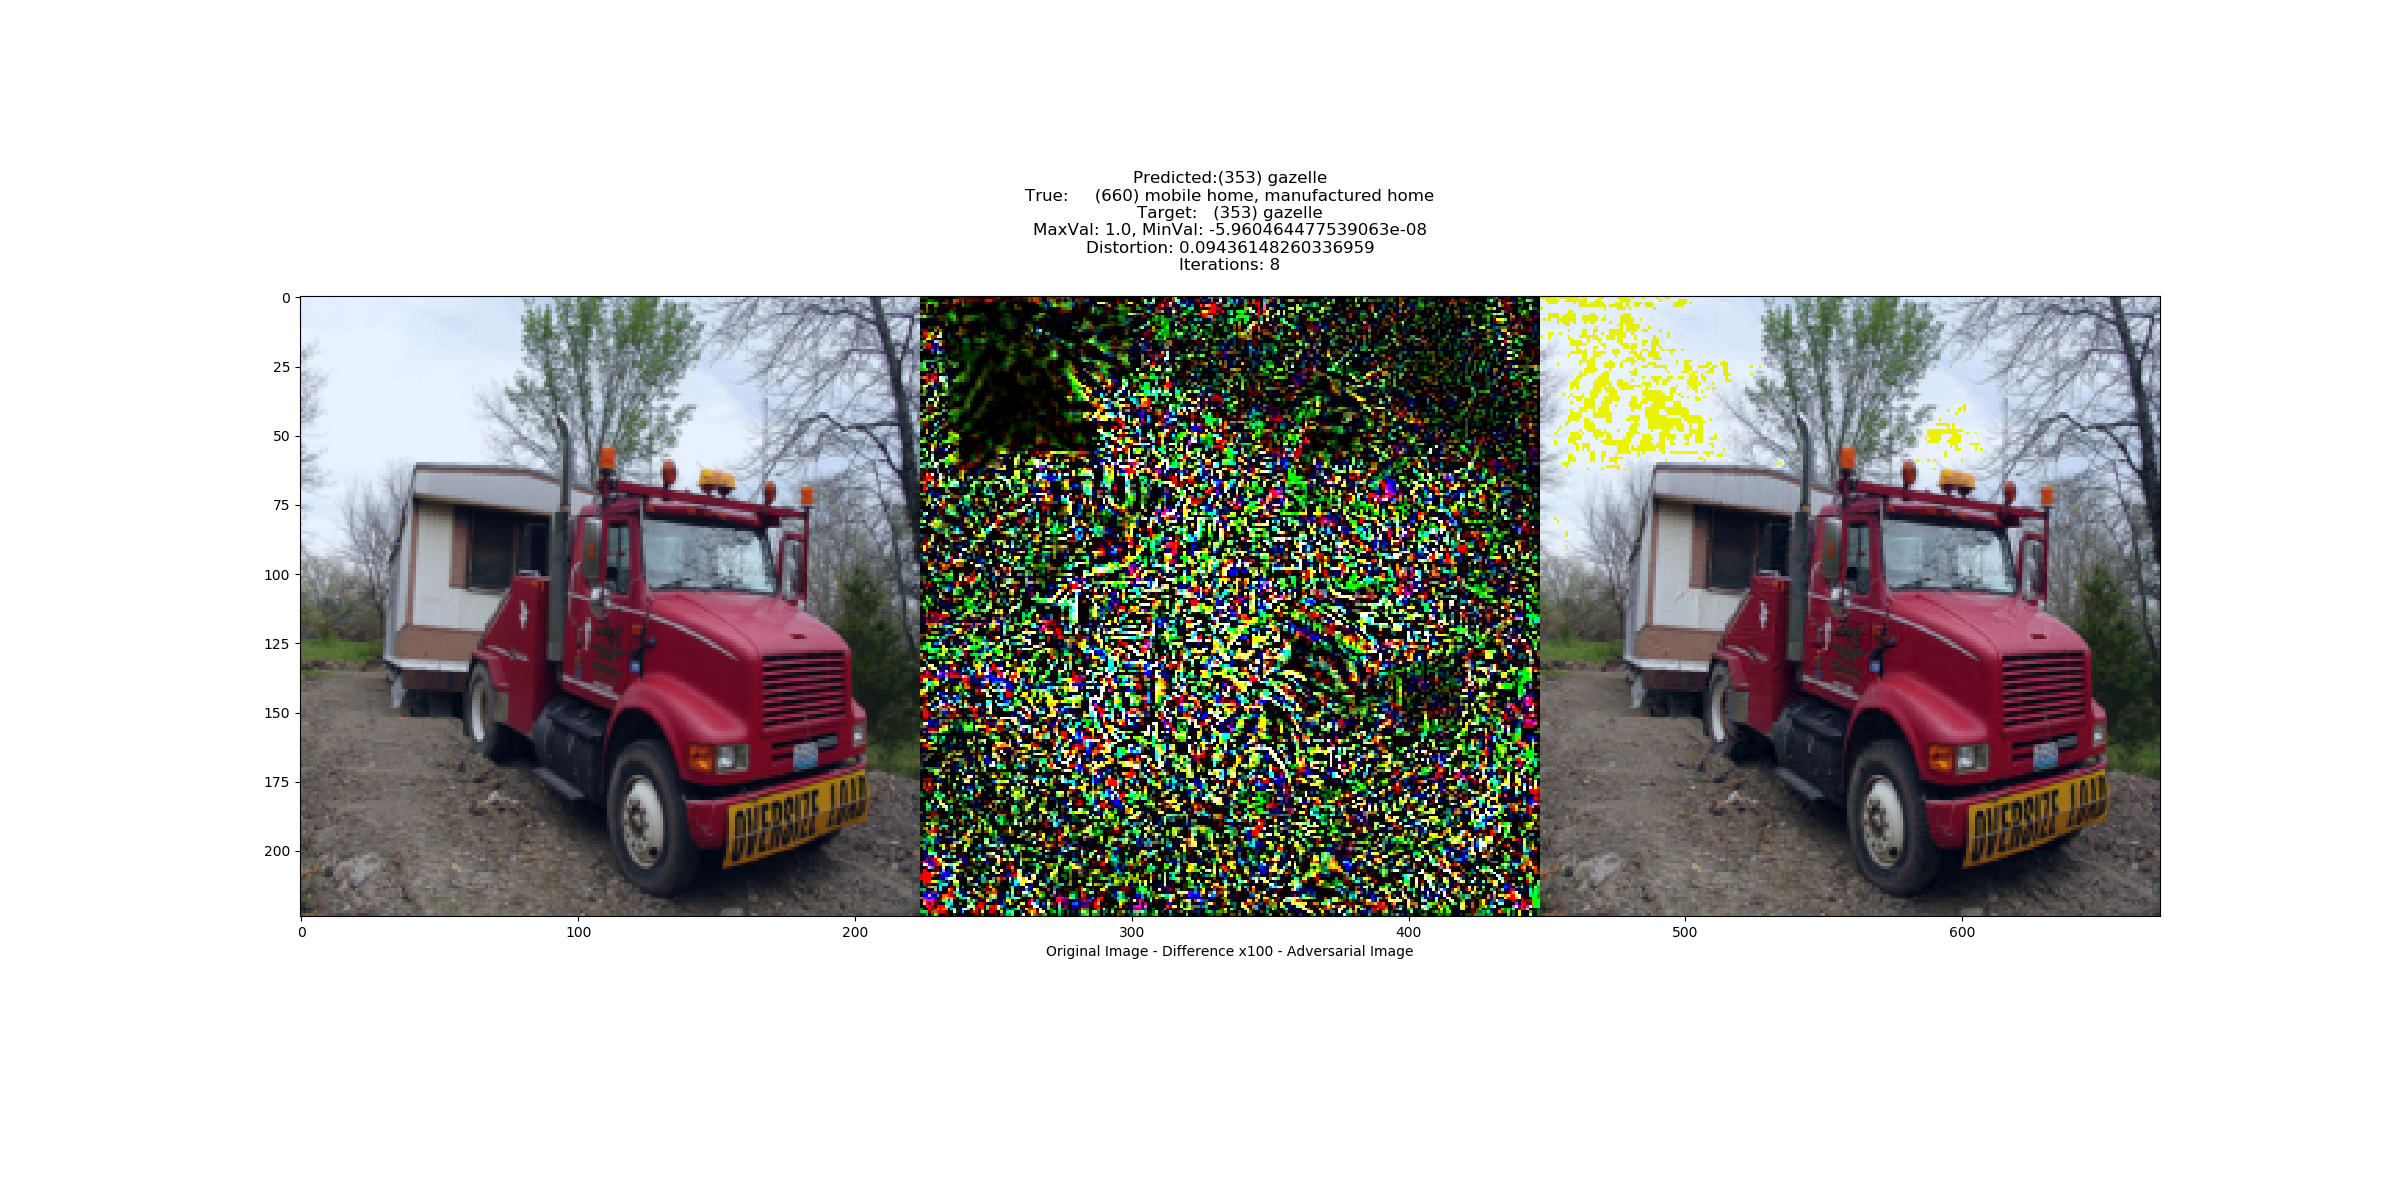
\includegraphics[width=7cm]{c1_figures/vgg16-ILSVRC2012_val_00035978-O803-A353-attack_summary.png}
% 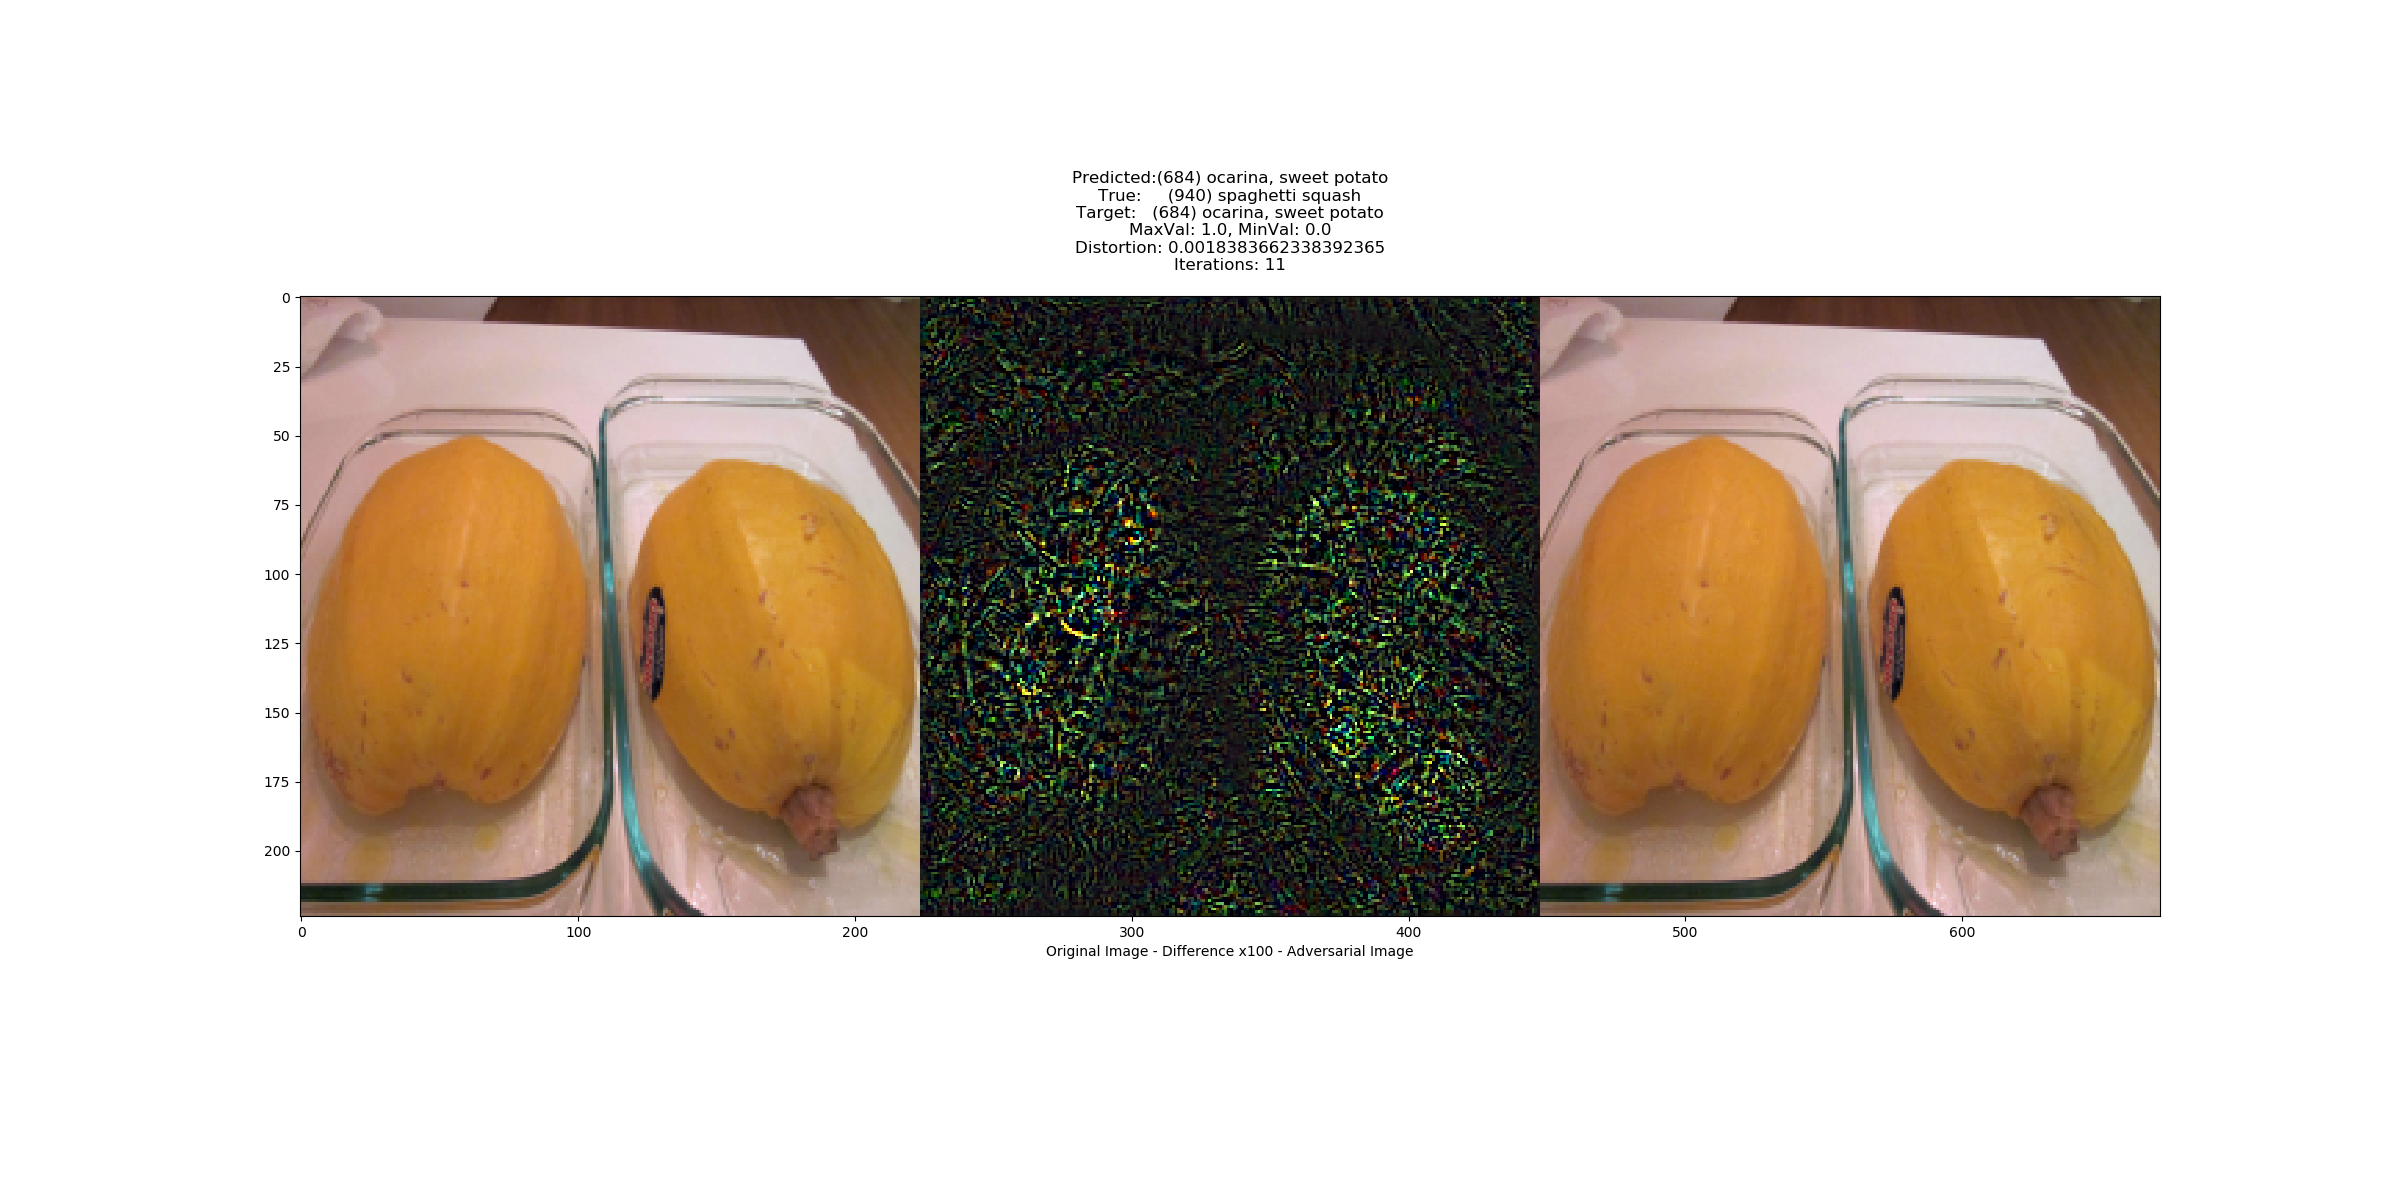
\includegraphics[width=7cm]{c1_figures/ILSVRC2012_val_00000886-Otensor([940])-A684-attack_summary.png}
\caption{Original images on the left, Perturbation (magnified by a factor of 100) by is in the middle, Adversarial Image (total of Original with Perturbation) is on the right. }
\end{figure}

%The average distortion was 0.01 distributed as seen in figure \ref{lbfgsi}. 

\begin{figure}[H]
\label{lbfgsi}
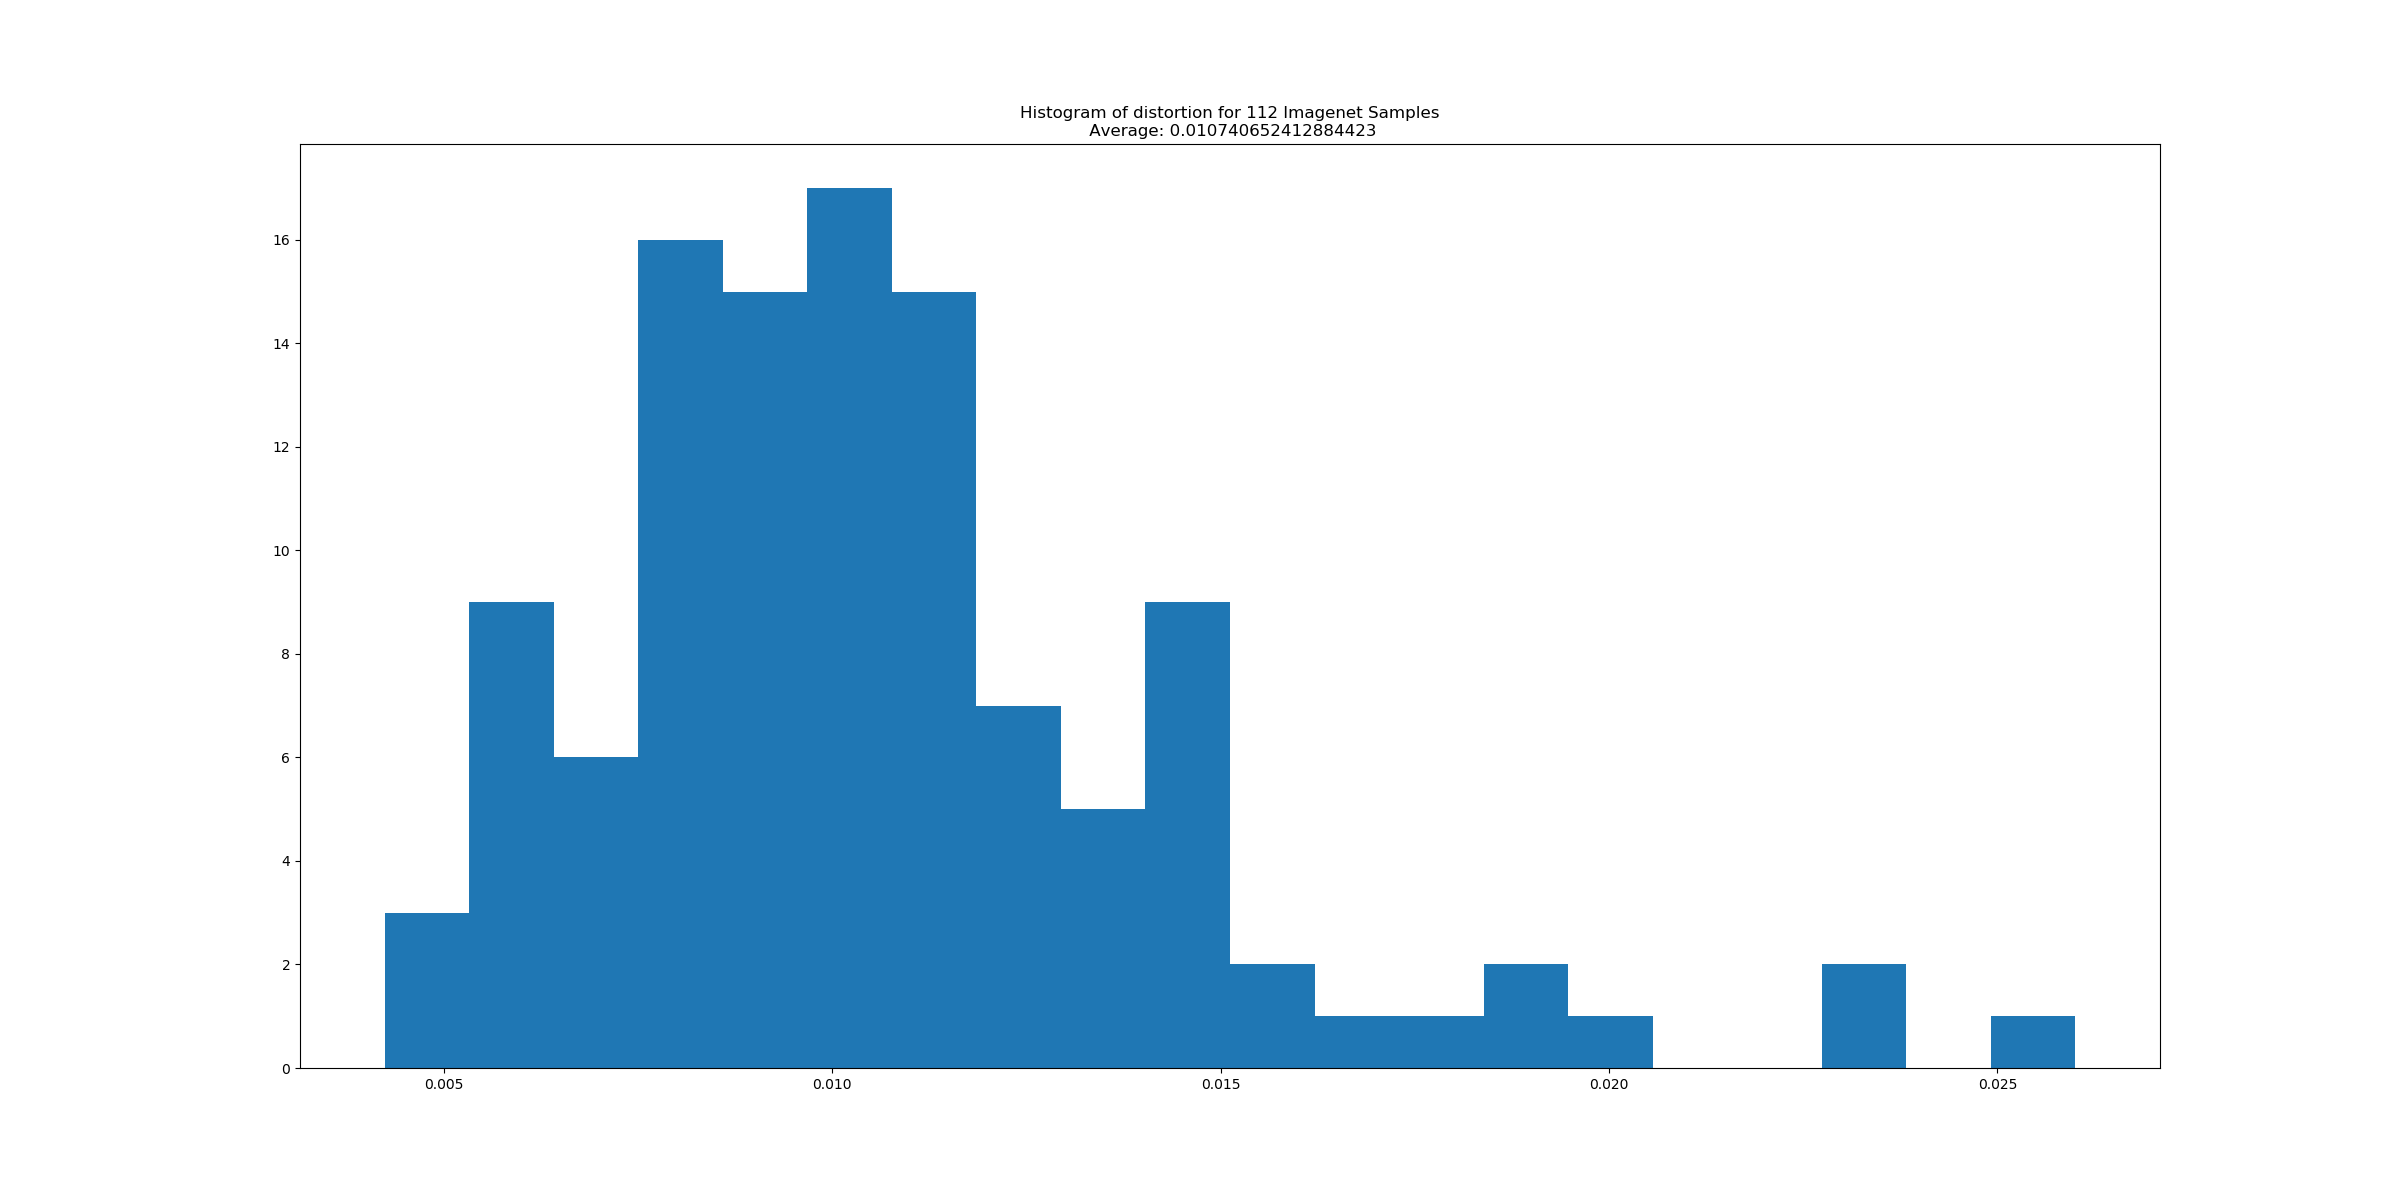
\includegraphics[trim=200 80 100 100, clip,width=14cm]{c1_figures/distortion_hist.png}
\caption{A histogram of the distortion measured for each of 112 adversarial examples generated using L-BFGS against the VGG16 network on ImageNet images with mean distortion 0.0107}
\end{figure}

\paragraph{Fast Gradient Sign Method (FGSM)} 

  We also implemented a single step attack process uses the gradient of the loss function $L$ with respect to the image to find the adversarial perturbation \cite{goodfellow_explaining_2014}. for given $\e$, the modified image $\hat x$ is computed as
\begin{equation}
\hat{x} = x + \epsilon \text{sign} (\nabla L (P_w(x),x))
\end{equation}

This method is simpler and much faster to compute than the L-BFGS technique described above, but produces adversarial examples less reliably and with generally larger distortion. Performance was similar but inferior to the Iterative Gradient Sign Method summarized below.  
%\[\hat x = x + \e \sign(\Delta \ell(F(x'_m),x'_m))\]

\paragraph{Iterative Gradient Sign Method (IGSM)}
\label{igsm-s}
In \cite{kurakin_adversarial_2016}
  an iterative application of FGSM was proposed. After each
  iteration, the image is clipped to a $\e L_\infty$ neighborhood of the original. Let $x'_0 = x$, then after $m$ iterations, the adversarial image obtained is:
\begin{equation}
x_{m+1}' = \text{Clip}_{x,\epsilon} \Bigl\{x_m' + \alpha \times \text{sign}(\nabla \ell (F(x'_m),x'_m))  \Bigr\} 
\label{igsm}
\end{equation}
This method is faster than L-BFGS and more reliable than FGSM but still produces examples with greater distortion than L-BFGS. 
%  \[x'_{m + 1} = \text{Clip}_{x,\e} \{ x'_m + \alpha \times
%  \sign(\Delta \ell(F(x'_m),x'_m))\] 
\begin{figure}[H]
  \centering
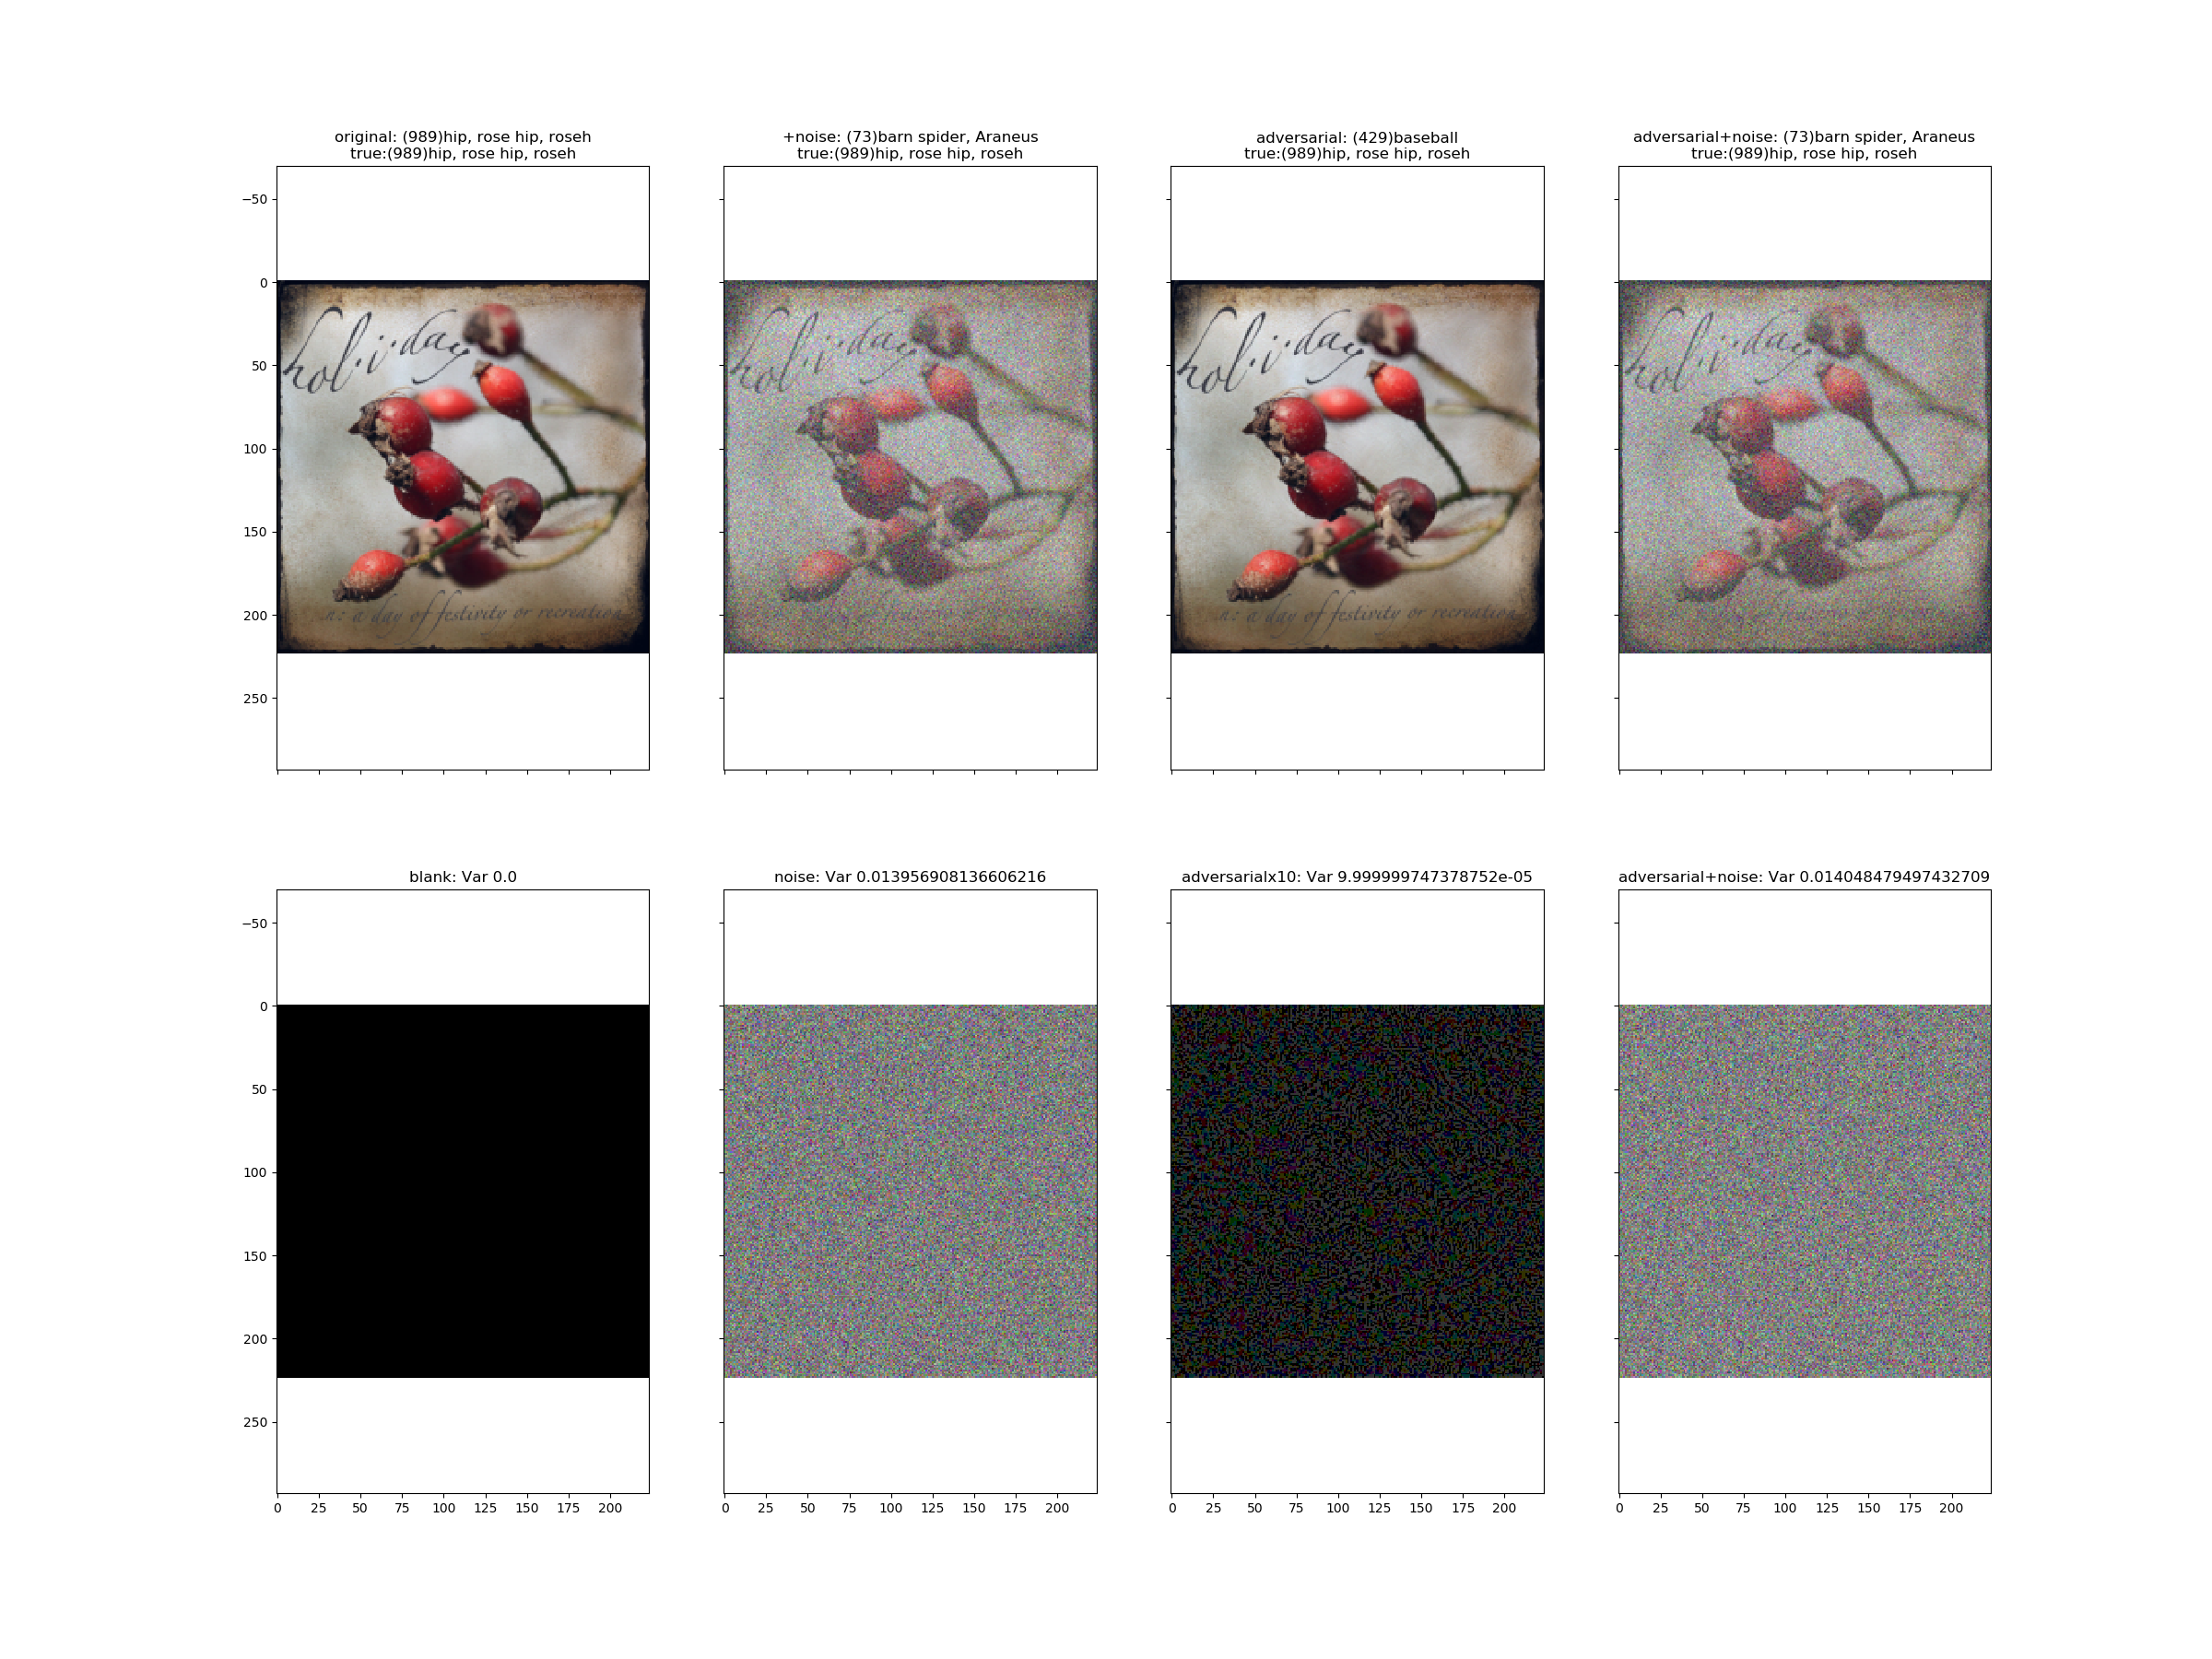
\includegraphics[trim=200 110 1200 102, clip,width=4cm]{c1_figures/ILSVRC2012_val_00002900summary_plot.png}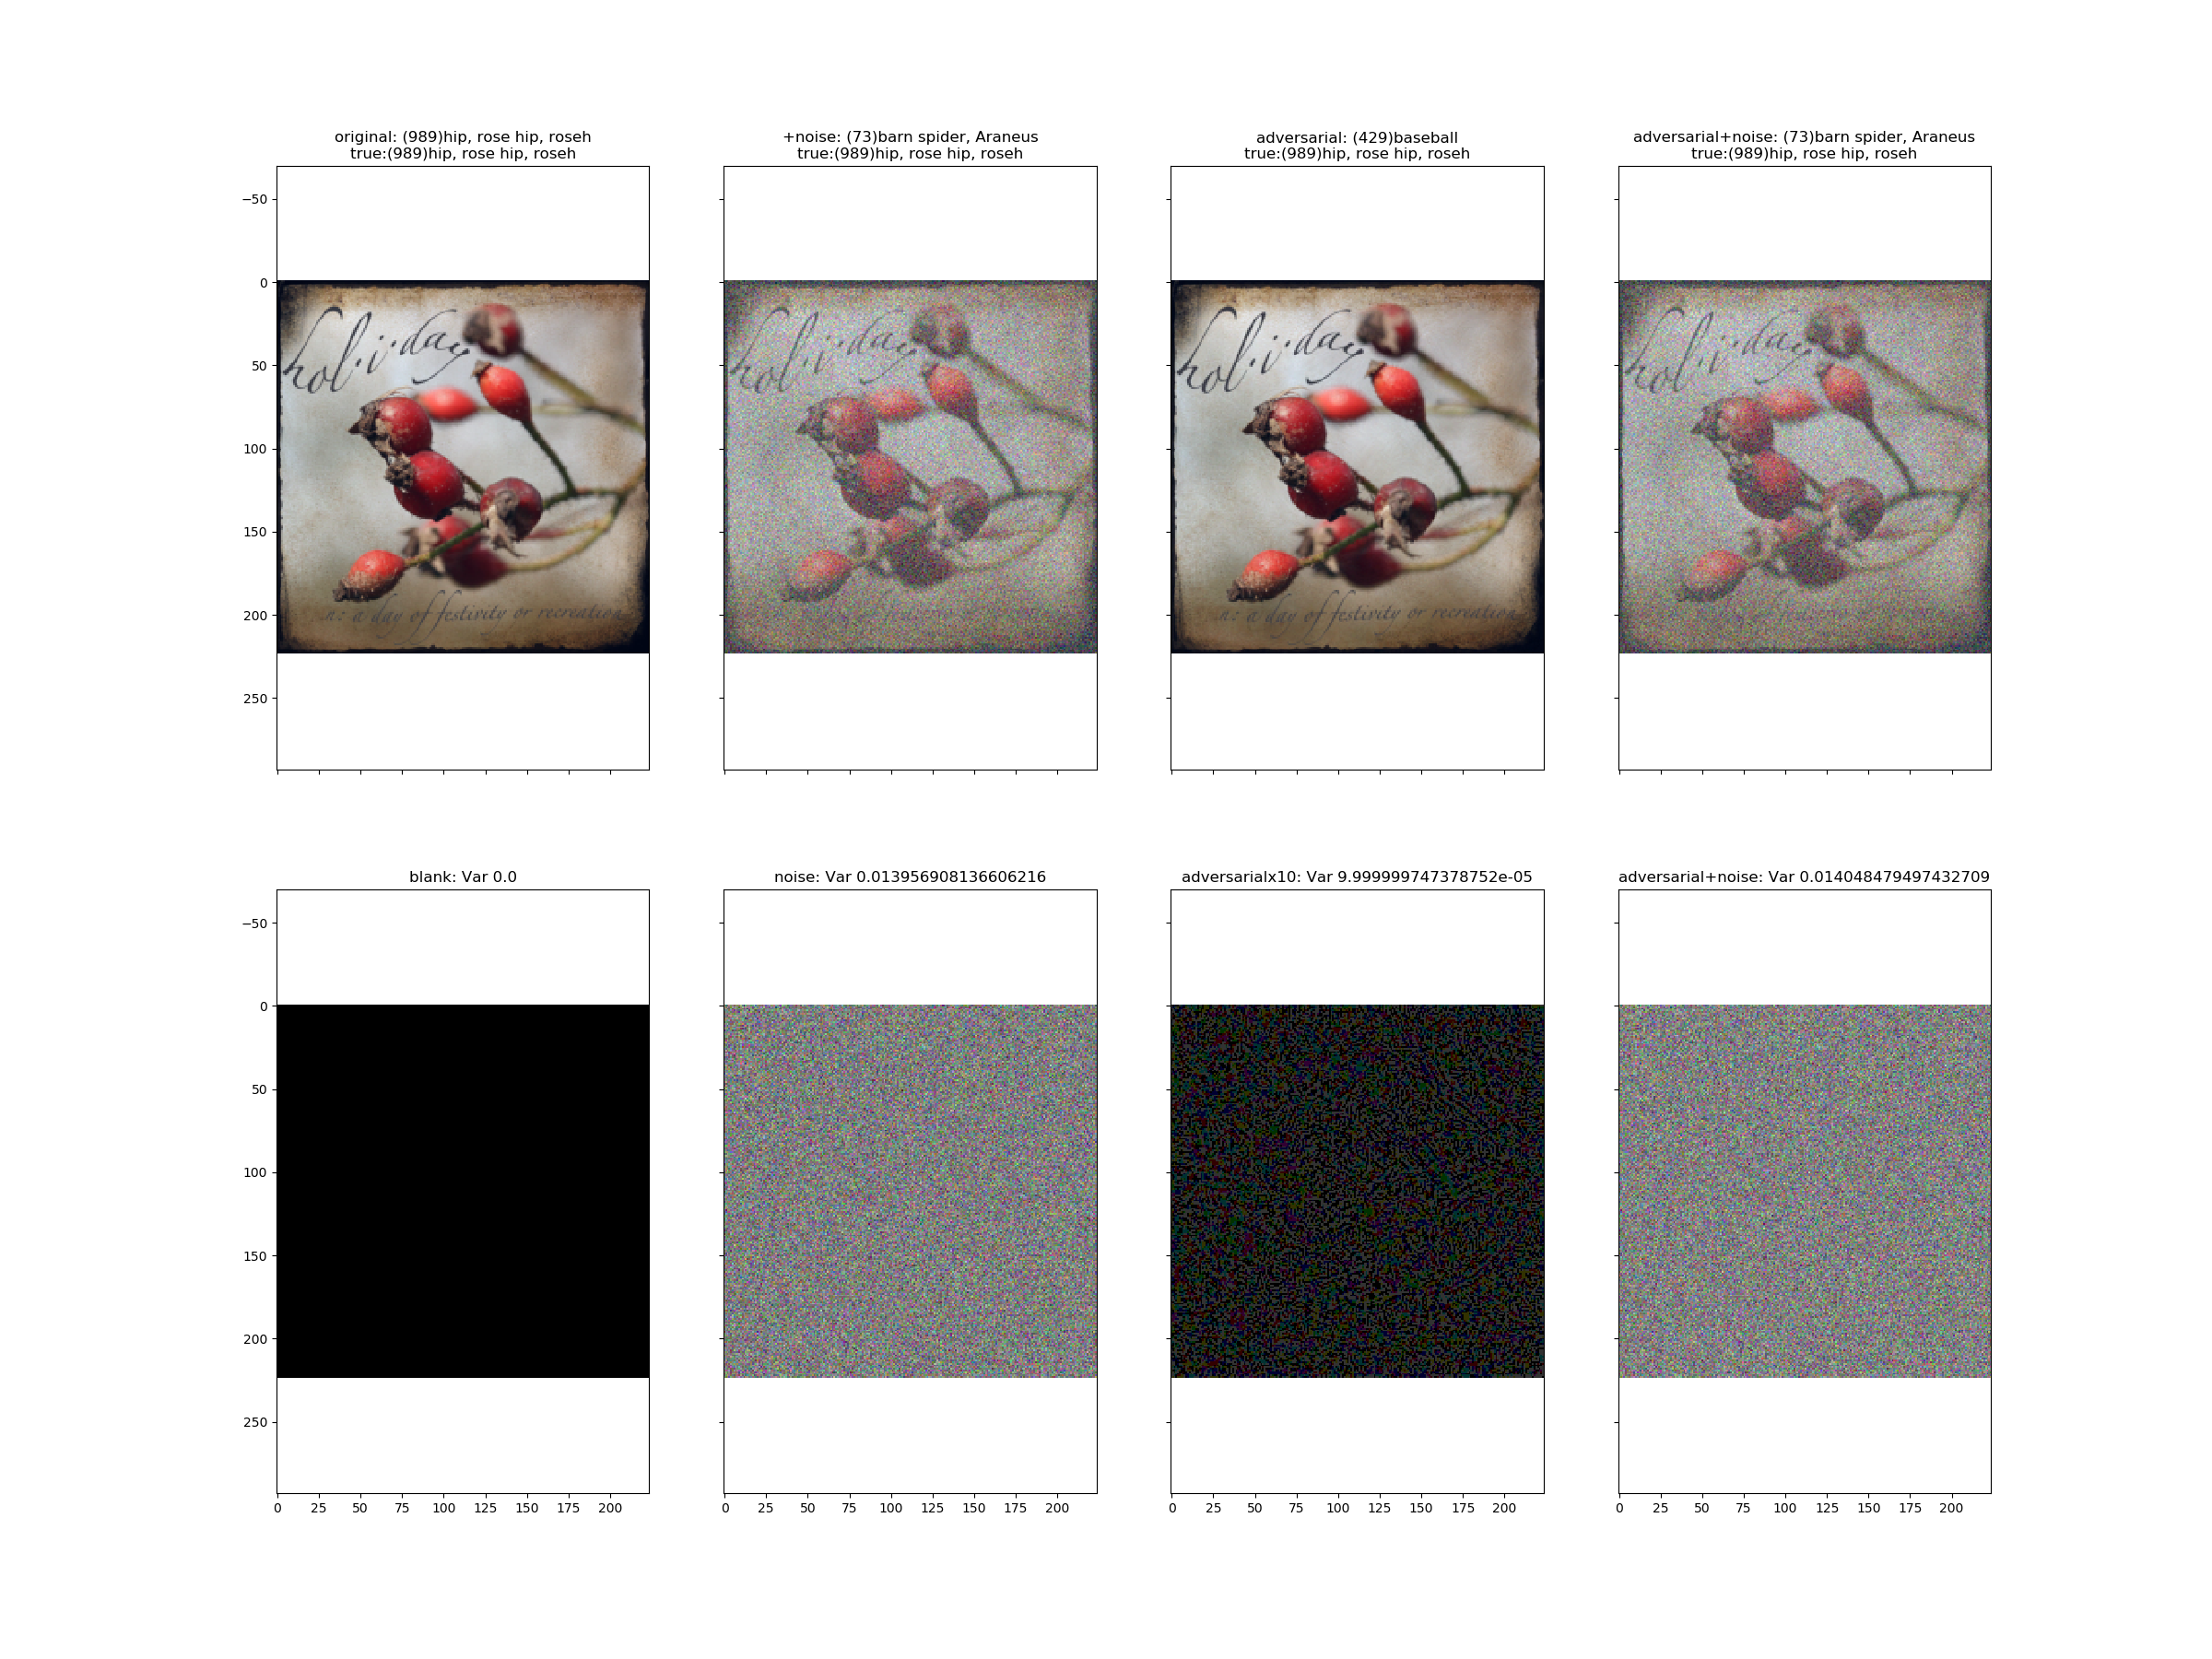
\includegraphics[trim=900 110 500 102, clip,width=4cm]{c1_figures/ILSVRC2012_val_00002900summary_plot.png}
%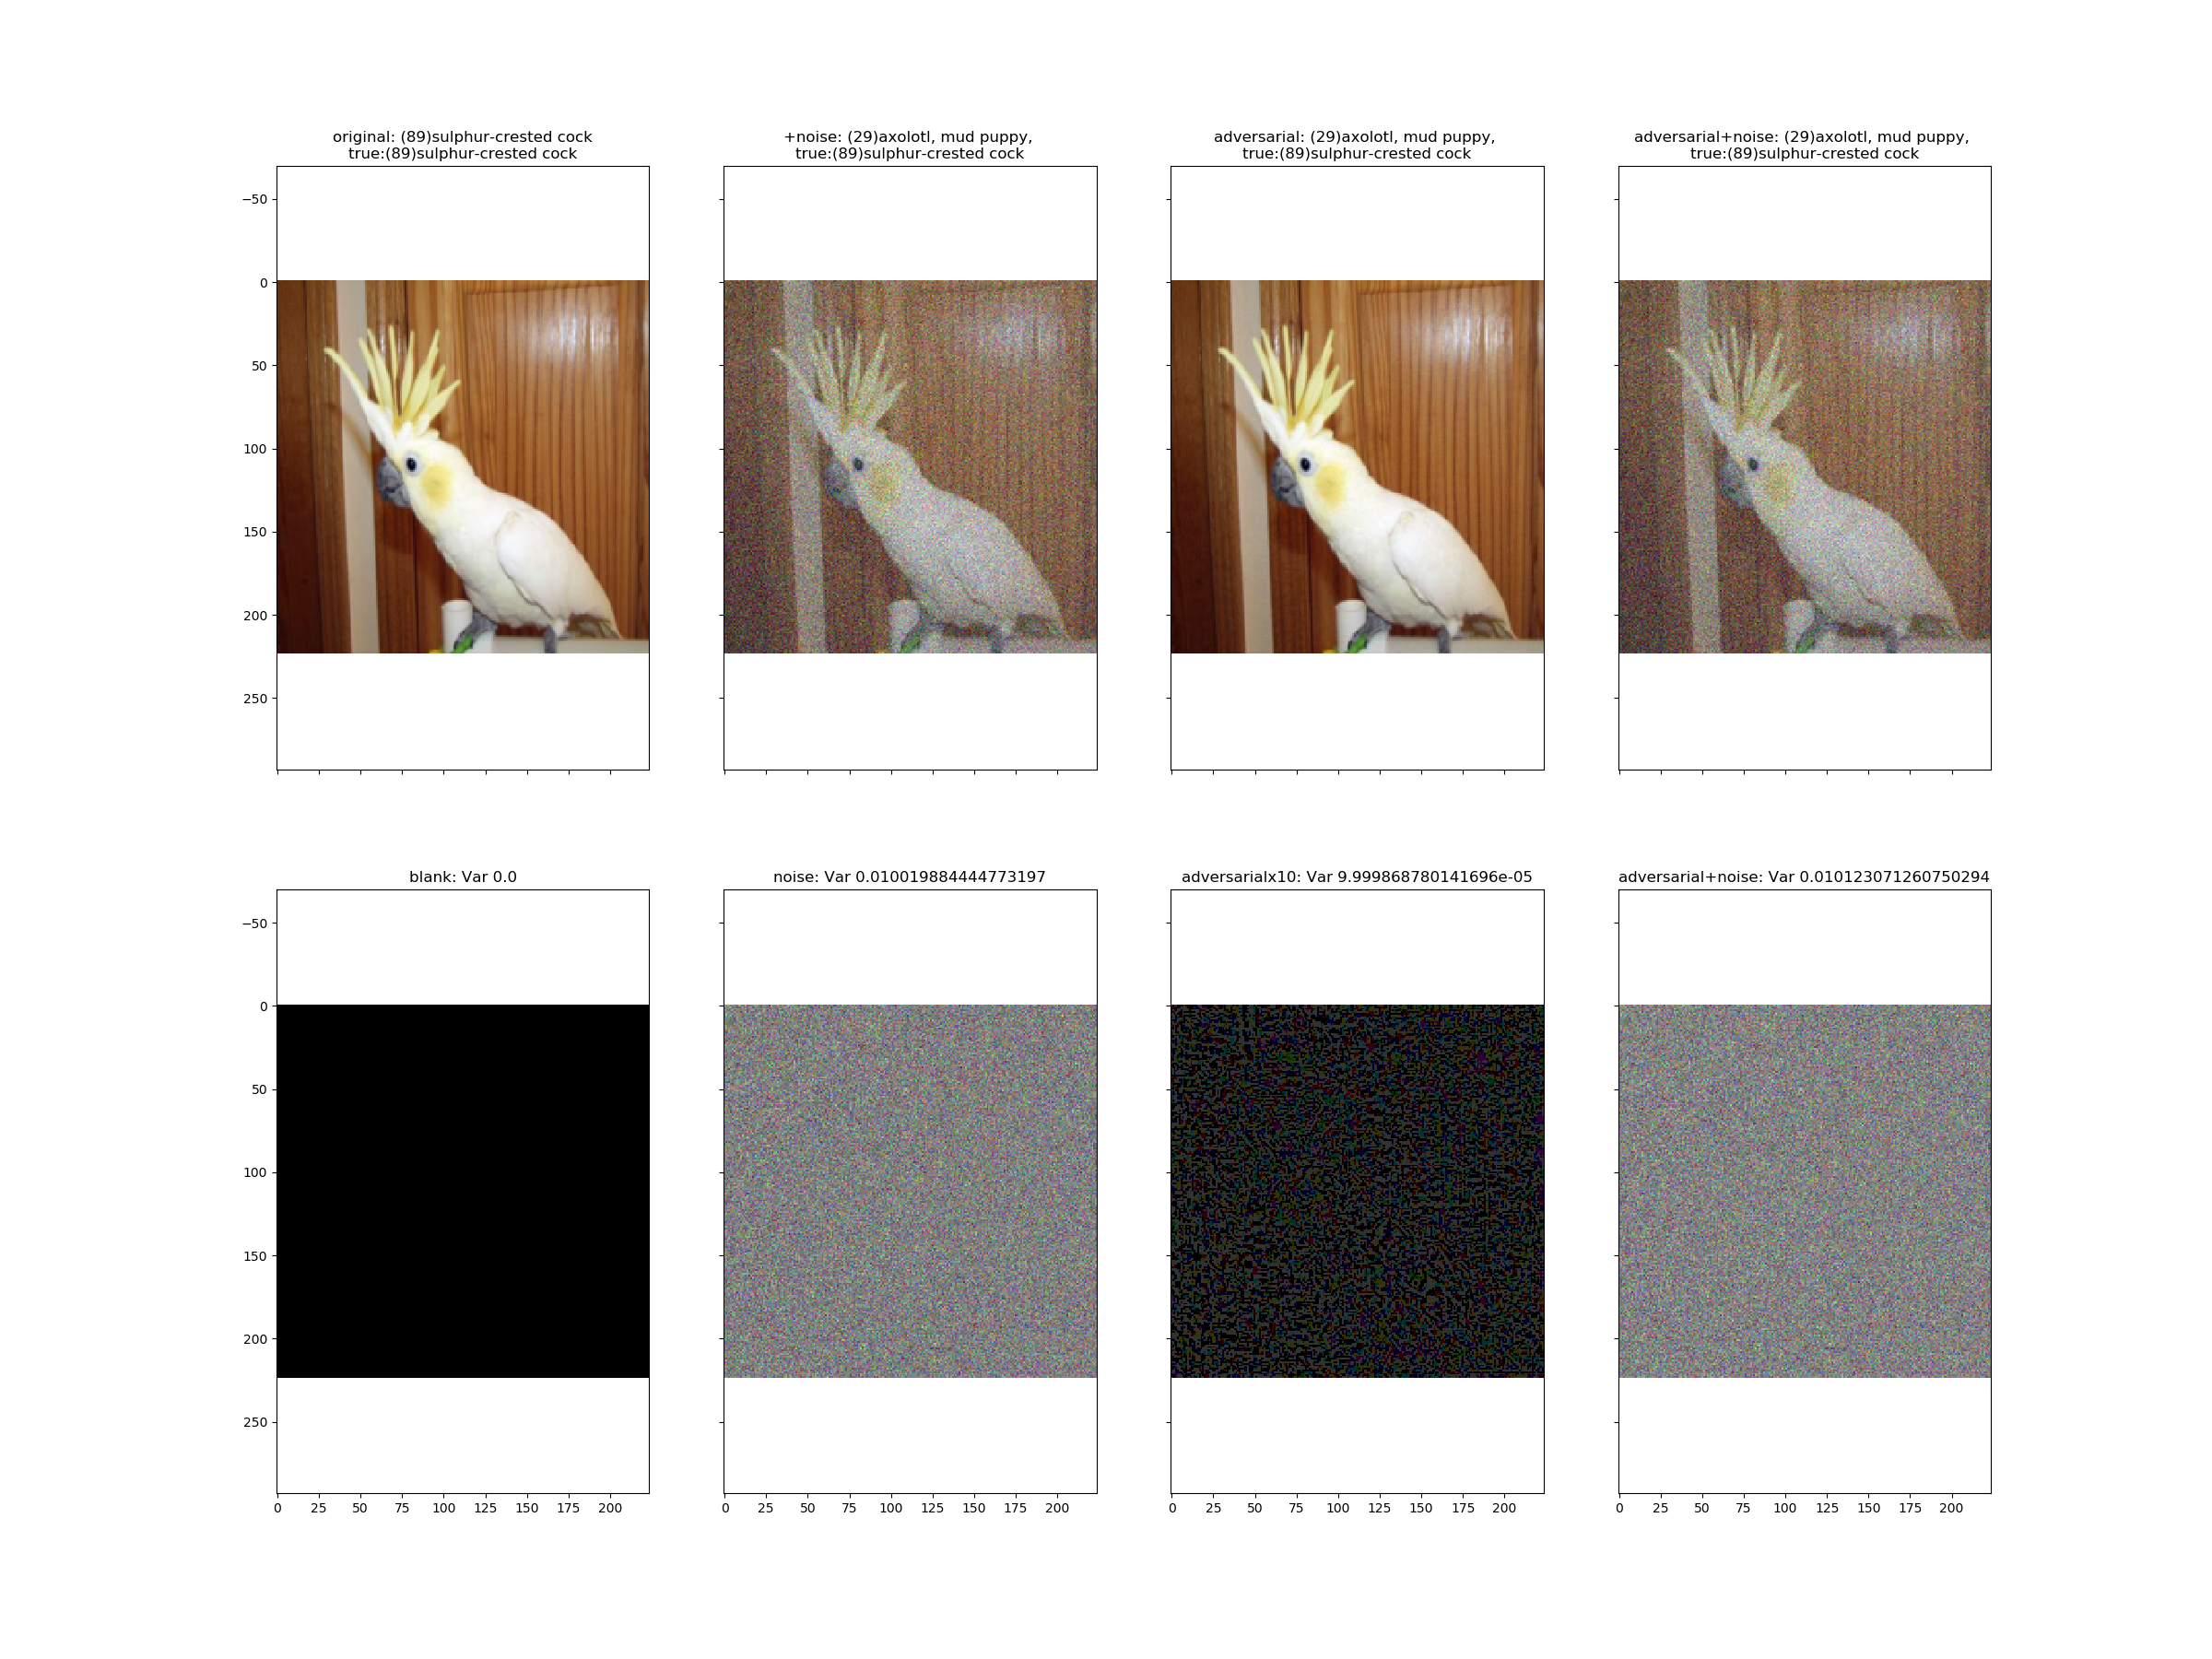
\includegraphics[width=12cm]{c1_figures/ILSVRC2012_val_00048234summary_plot.png}
\label{fgsmhip}
\caption{adversarial example generated against VGG16 (ImageNet) with IGSM. Original Image on the left, adversarial image and added noise (ratio of variance adversarial noise/original image: 0.0000999) on the right. }
\end{figure}

%The attacks contained in figure ~\ref{fgsmhip} were generated with IGSM against VGG16


\subsection{Other Attacks}
The following attack techniques are also prevalent in the literature but have not been replicated in these experiments. 

\paragraph{Jacobian-based Saliency Map Attack (JSMA)} Another attack noted by  \cite{papernot_limitations_2015}
  estimates the \emph{saliency map}, a rating for each of the input features (e.g. each pixel) on how influential it is for causing the model to predict a particular class with respect to the model output \cite{wiyatno2018saliency}. This attack modifies the pixels that are most salient. This is a targeted attack, and saliency is designed to find the pixel which increases the classifier's output for the target class while tending to decrease the output for other classes.

\paragraph{Deep Fool (DFool)} A technique proposed by \cite{moosavi-dezfooli_deepfool:_2015}
  to generate an un-targeted iterative attack. 
This method approximates the classifier as a linear decision boundary and then finds the smallest perturbation needed to cross that boundary.
This attack minimizes $L_2$ norm with respect to  to the original image.

\paragraph{Carlini \& Wagner (C\&W)} In \cite{carlini_towards_2016}
  an adversarial attack is proposed which updates the loss function such that it jointly minimizes $L_p$ and a custom differentiable loss function based on un-normalized outputs of the classifier (\textit{logits}). 
Let $Z_k$ denote the logits of a model for a given class $k$, and $\kappa$ a margin parameter. Then C\&W tries to minimize:
\begin{equation}
|| x - \hat{x} ||_p + c* max\left(Z_k(\hat{x}_y) - max\{Z_k(\hat{x}) : k \neq y\},-\kappa\right)
\end{equation}


\section{Theory of Adversarial Examples}

% summarize:
% odds are odd
% features not bugs (and rebuttal?)
% dimpled manifolds

~\cite{roth19aodds} proposed a statistical method to identify adversarial examples from natural data. Their main idea was to consider how the last layer in the neural network (the logit layer) would behave on small perturbations of a natural example. %, i.e., on $x+\varepsilon n$ where $x$ is a natural example, $\varepsilon>0$ is small, and $n \sim N(0,I)$.  
This is then compared to the behavior of a potential adversarial example. If it differs by a predetermined threshold, the example is flagged as adversarial. Successfully flagging adversarial examples in this way works best when adversarial examples tend to perturb toward the original class from which the adversarial example was perturbed. However, this is not always the case.
It was shown by ~\cite{hosseini2019odds} that it is possible to produce adversarial examples, for instance using a logit mimicry attack, that instead of perturbing an adversarial example toward the true class, actually perturb to some other background class. In fact, we will see in Section \ref{sec:mnist} that the emergence of a background class, which was observed as well by ~\cite{roth19aodds}, is quite common. 

Whereas ~\cite{roth19aodds} consider adding various types of noise to a given point and ~\cite{hosseini2019odds} consider small Gaussian perturbations of $x$ sampled from $N(x,\varepsilon^2 I)$ for small $\varepsilon$, %\todo{[K]: Should we go ahead and just be clear here and say $N(x,\varepsilon^2 I)$?} %noise perturbations of $\varepsilon$ times a vector with normal distribution $N(0,I)$ with a small selection of choices for $\varepsilon.$
we specifically focus on %Our choice to consider varying standard deviations is quite similar to considering varying choices of $\varepsilon$ in the latter, but our focus is on 
tuning the standard deviation parameter to determine a statistic describing how a given data point is placed within its class. The $\gamma$-persistence then gives a measurement similar to distance to the boundary but that is drawn from sampling instead of distance. The sampling allows for a better description of the local geometry of the class and decision boundary, as we will see in Section \ref{sec:stab}. Our statistic is based on the fraction of a Gaussian sampling of the neighborhood of a point which receives the same classification; this is different from that of ~\cite{roth19aodds}, which is the expected difference of the output of the logit layer of the original data point and the output of the logit layer for perturbed data points.  Additionally, while their statistics are defined pairwise with reference to pre-chosen original and candidate classes, ours is not.

%%%%%%%%%%%%%%%%%%%%%%%%%%%%%%%%%%%%%%%%%%%%%%%%%%%%%%%%%%%%%%%%%%%%%%%%%%%%%%%%%%%%%%%%%%%%%%%%%%%%%%%%%%%%%%%%%%%%%%%%%%%%%%%%%%%%%%%%%%%%%%%%%%%%%%%%%%%%%%%%%%%%%%%%%%%%%%%%%%%%%%%%%%%%%%%%%%%%%%%%%%%%%%%%%%%%%%%%%%%%%%%%%%%%%%%%%%%%%%%%%%%%%%%%%%%%%%%%



